\documentclass[journal,twoside,web]{ieeecolor}

\usepackage{generic}
\usepackage{cite}
\usepackage{amsmath,amssymb,amsfonts}
\usepackage{algorithmic}
\usepackage{graphicx}
\usepackage{adjustbox}
\usepackage{booktabs}
\usepackage{multirow}
\usepackage{textcomp}
\usepackage{url}

\def\BibTeX{{\rm B\kern-.05em{\sc i\kern-.025em b}\kern-.08em
    T\kern-.1667em\lower.7ex\hbox{E}\kern-.125emX}}

\markboth{\journalname, VOL. XX, NO. XX, XXXX}
{Author \MakeLowercase{\textit{et al.}}: WindFormer for Short-Term Wind Resource Forecasting}

\begin{document}

\title{WindFormer: A Common-Speed and Direction-Vector Network for Wind Resource Forecasting}

\author{First A. Author, Second B. Author, and Third C. Author
\thanks{Manuscript received Month XX, 2026; revised Month XX, 2026.}
\thanks{The authors are with the corresponding institutions. Corresponding author: Author Name.}}

\maketitle

\begin{abstract}
Accurate short-term wind resource forecasting is critical for wind farm dispatch and power system operation. However, existing methods face distinct limitations when handling different wind variables. For wind speed, they typically model cross-turbine interactions using a single dependency pattern, which overlooks shared meteorological dynamics. For wind direction, they often treat angles as ordinary one-dimensional scalars, ignoring the discontinuity at periodic boundaries. To address these issues, we propose WindFormer, a common-speed and direction-vector network for wind resource forecasting. The wind-speed branch extracts a learnable common wind field from multiple turbines, combining Phase-Attention with residual modeling to capture shared evolutionary trends and turbine-specific deviations. Concurrently, the wind-direction branch transforms each direction angle into a two-dimensional sine-cosine unit-vector representation and employs turbine-wise shared Patch Attention. These predictions are further regularized by direction-vector consistency and wind-vector consistency losses to preserve boundary continuity. On two real-world wind farm datasets with different periodic characteristics and spatial distributions, WindFormer achieves consistent improvements. Compared with state-of-the-art baselines, it reduces MAE by 10.2\% for wind speed and 10.1\% for wind direction. Furthermore, in cross-turbine zero-shot experiments on the Penmanshiel dataset, WindFormer limits the relative degradation of wind-direction MAE to only +17.2\%, outperforming the strongest baseline's +20.3\%. This demonstrates its robust generalization on unseen turbines under complex spatio-temporal coupling conditions.
\end{abstract}

\begin{IEEEkeywords}
Spatio-temporal modeling, wind speed forecasting, wind direction forecasting, wind turbines, deep learning, time series forecasting.
\end{IEEEkeywords}

\section{Introduction}
\label{sec:introduction}

Driven by its clean nature and reliable supply, wind power has become an important energy source for modern power systems. Accurate wind speed and direction forecasting is essential for grid dispatch, resource allocation, and wind-energy utilization \cite{Hanifi2020CriticalReviewWindPowerForecasting,Jung2014CurrentStatusWindSpeedPowerForecasting}. However, existing methods typically process different wind speed and direction using a single, unified approach. This approach overlooks a critical physical reality: wind speed and wind direction possess fundamentally distinct cross-turbine structures and mathematical properties \cite{Chen2014WindPowerForecastsGaussianProcesses,Dolatabadi2022DeepSpatialTemporal2DCNNBLSTM}.

As illustrated in Fig.~\ref{fig:data_properties}, wind speed and wind direction show different modeling properties. First, wind speed exhibits a strong shared property: because the turbines are driven by similar weather patterns, their trajectories usually follow comparable trends. Therefore, effective wind-speed modeling should leverage these shared dynamics.


\begin{figure}[!t]
	\centering
	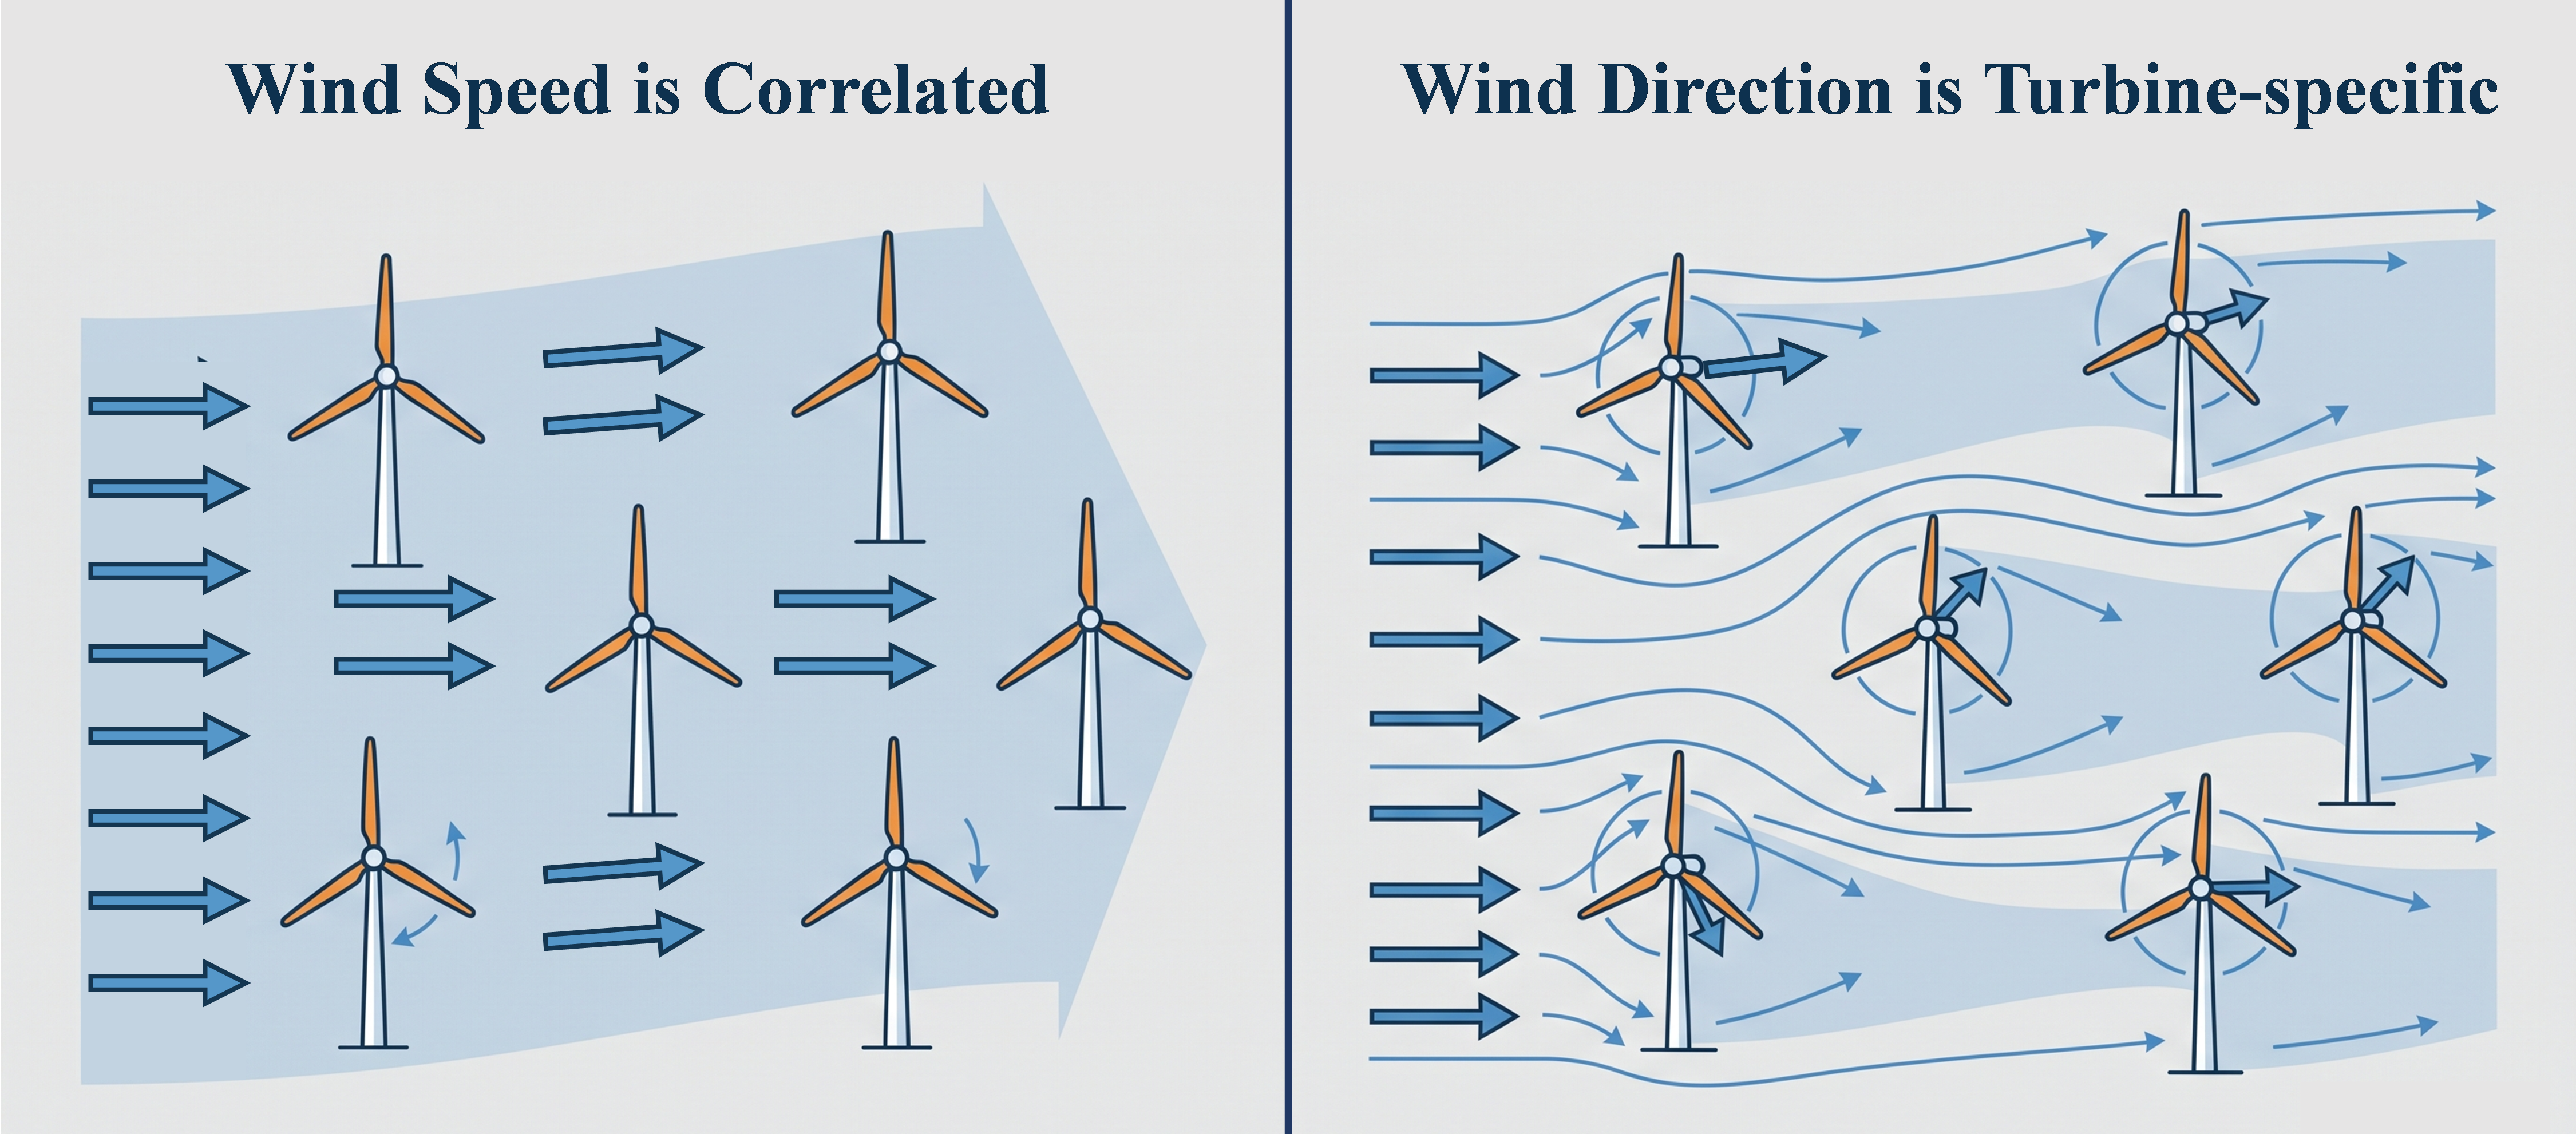
\includegraphics[width=0.48\textwidth]{figures/figure1.png}
	\caption{Conceptual contrast between cross-turbine wind-speed correlation and turbine-specific wind-direction variation.}
	\label{fig:data_properties}
\end{figure}

Second, wind direction presents different challenges. On the one hand, interactions among turbine spatial locations, wake effects, and local flow fields cause different units to exhibit distinct dominant directions and variation ranges. On the other hand, raw wind direction is usually recorded as a one-dimensional angle, which is discontinuous at the periodic boundary. For instance, $0^\circ$ and $360^\circ$ physically represent the same direction, and $359^\circ$ and $1^\circ$ differ by only $2^\circ$. If treated as a regular scalar, the model may misinterpret the latter as a massive $358^\circ$ separation. This misrepresentation turns physically continuous transitions into abrupt numerical jumps. Therefore, wind direction forecasting requires representations and error metrics that respect periodic continuity.

Based on the above observations, this paper focuses on the sharing property of wind speed and the periodic nature of wind direction, and further addresses two research questions(RQ):

\textbf{RQ1:}
How can we exploit the shared wind-speed dynamics among multiple turbines?

\textbf{RQ2:}
How can we preserve boundary continuity in wind-direction signals?

Driven by this motivation, we conduct an in-depth exploration of the two research questions detailed below.

\subsection{Wind Speed Forecasting}
\label{subsec:speed_sharing_intro}

Multiple turbines are affected by similar weather processes and large-scale wind fields, but local terrain and wake effects still produce turbine-level deviations. Channel-independent methods preserve these differences but repeatedly relearn common variations, whereas fully correlated methods may mix common and local dynamics. We therefore extract a shared wind field and model turbine-specific residuals separately.

Fig.~\ref{fig:speed_multiscale_similarity} further shows that representative turbines exhibit similar dominant frequency components and wavelet energy patterns, supporting the existence of shared multi-scale wind-speed dynamics across turbines.

\begin{figure}[!t]
\centering
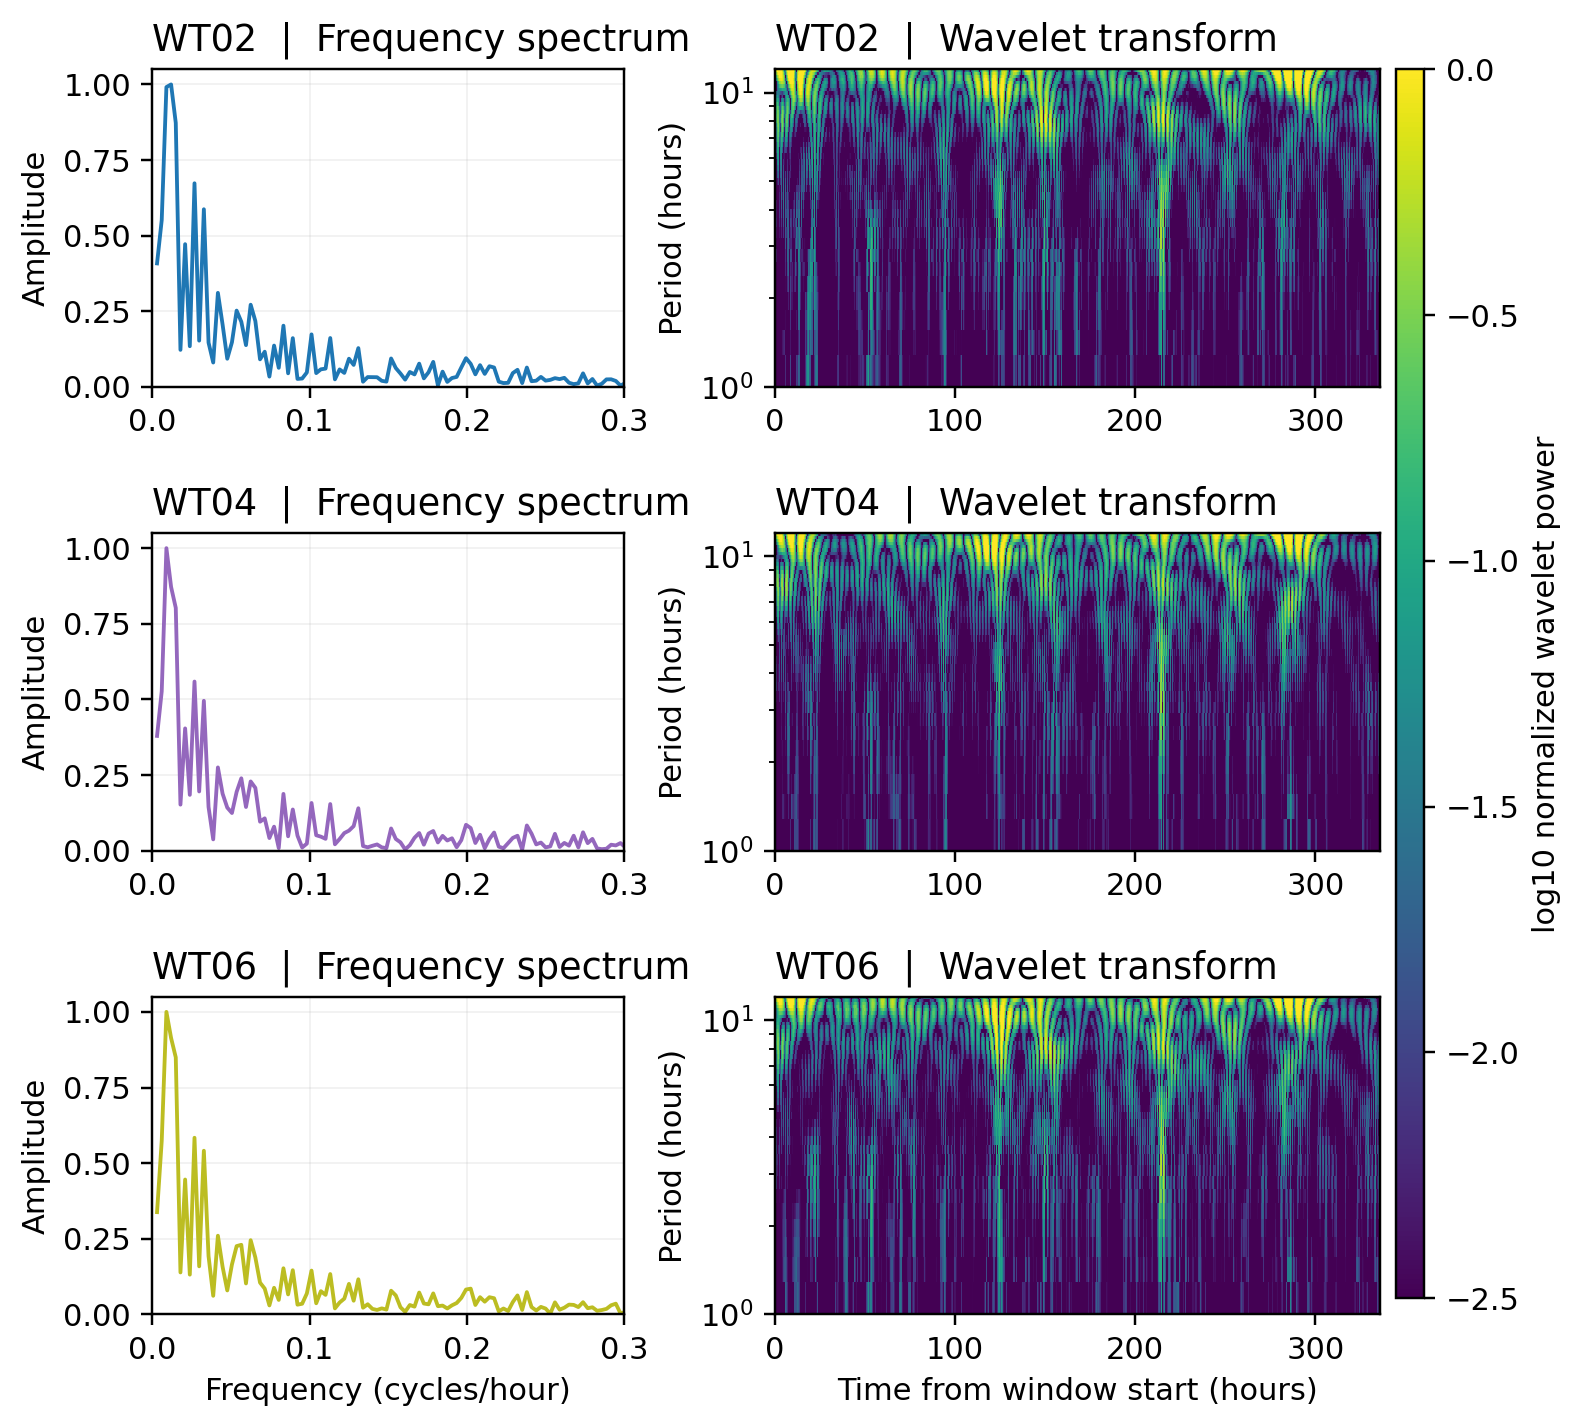
\includegraphics[width=0.48\textwidth]{figures/figure2.png}
\caption{Frequency-spectrum and wavelet-transform comparison of representative turbine wind-speed sequences. Similar dominant frequency components and wavelet energy patterns support the shared multi-scale dynamics of wind speed across turbines.}
\label{fig:speed_multiscale_similarity}
\end{figure}

After extracting the common wind field, we introduce a Phase representation. By aligning observations at similar evolutionary stages, this approach effectively captures periodic wind dynamics and mitigates distribution drift across time blocks.

\subsection{Wind Direction Forecasting}
\label{subsec:direction_2d_intro}

Wind speed and wind direction have different cross-turbine structures. The interaction among turbine locations, wakes, and local flow fields causes different units to present distinct dominant directions and turning patterns, so wind direction should not be collapsed into a common representation in the same way as wind speed. Fig.~\ref{fig:direction_specificity} (a) shows that the dominant directions and directional concentration levels of different turbines are not consistent. Fig.~\ref{fig:direction_specificity} (b) reveals that about 51\% of turbine pairs have an average angular distance of no less than $90^\circ$, indicating that cross-turbine directional differences are not caused by a few outliers. Fig.~\ref{fig:direction_specificity} (c) further displays the difference structure among 24 turbines using a pairwise angular distance matrix, where high and low angular distances alternate across regions, demonstrating that wind-direction relationships exhibit strong turbine-level dependence. Therefore, wind-direction modeling needs to preserve turbine-specific directional information.

\begin{figure}[!t]
\centering

\includegraphics[width=0.48\textwidth]{figures/all_24_turbines_direction_difference_summary.png}
\caption{Turbine-specific wind direction distributions and all-pair angular differences among 24 turbines.}
\label{fig:direction_specificity}
\end{figure}

In addition, wind direction is not a regular one-dimensional scalar because its numerical boundary is physically connected. Wind direction satisfies

\begin{equation}
\theta \equiv \theta+360^\circ.
\end{equation}

Direct scalar regression breaks this equivalence near the boundary and may distort distances, local variations, and error gradients. Thus, wind direction forecasting must preserve boundary continuity from the input representation, rather than merely correcting angles after prediction. To this end, this paper maps the one-dimensional direction angle of each turbine into a two-dimensional sine-cosine unit-vector representation:

\begin{equation}
\mathbf{u}_{t,n} = [\cos(\theta_{t,n}), \sin(\theta_{t,n})].
\end{equation}

This mapping keeps boundary-adjacent directions close to each other in the representation space and provides unified coordinates for subsequent forecasting and error calculation. On this basis, the model performs predictions in the two-dimensional direction space, uses direction-vector loss and vector-consistency loss to constrain the prediction results, and then restores the predicted components to angles:

\begin{equation}
\hat{\theta}_{t,n} = \operatorname{atan2} \left( \hat{u}^{\sin}_{t,n}, \hat{u}^{\cos}_{t,n} \right)
\end{equation}

For wind-direction forecasting, we segment the two-dimensional direction sequence of each turbine into patches and extract local temporal patterns using shared Patch Attention. Specifically, the sine-cosine representation resolves the boundary discontinuity by defining continuous directional coordinates and distance metrics, while the patch strategy structures the historical temporal sequences. Because dominant directions and turning patterns vary significantly across units, the wind-direction branch processes inputs and outputs on an individual turbine basis. However, since local temporal dynamics often contain transferable structures, all turbines share the same patch-attention module. This architecture prevents the inappropriate compression of distinct wind directions into a single global state while enabling shared temporal modeling within a physically consistent two-dimensional representation space.

\subsection{WindFormer Framework}

Based on these issues, this paper constructs WindFormer as a common-speed and direction-vector learning framework. For the wind-speed branch, WindFormer first extracts common wind-field dynamics from the wind speeds of multiple turbines through learnable weighted aggregation, treating the independent variation of each turbine as a local residual. Subsequently, the common wind field is modeled via attention using Phase as the basic unit, while local residuals are refined by lightweight MLPs. For the wind-direction branch, WindFormer first converts each one-dimensional direction angle into sine-cosine components to eliminate boundary discontinuities and then extracts directional variation patterns through turbine-wise Patch sequences and shared Patch Attention. The two branches remain structurally decoupled and are trained jointly through a unified loss.

The main contributions of this paper are as follows:

\begin{itemize}
	\item \textbf{In terms of wind-speed modeling, we propose a common-wind-field modeling strategy.} This method first extracts cross-turbine shared wind-field dynamics and then models the independent local variations of each turbine. To represent recurring variation processes within the common wind field, we introduce Phase representation to align similar cross-period processes.
    \item \textbf{In terms of wind-direction modeling, we propose a two-dimensional unit-vector representation strategy for multi-turbine wind direction forecasting.} Because raw wind direction is a one-dimensional angle with boundary discontinuity, we retain turbine-wise wind direction sequences and adopt sine-cosine components to describe distribution differences and directional variation patterns more faithfully.
    \item \textbf{We develop and comprehensively evaluate a structure-aware dual-branch forecasting algorithm.} WindFormer jointly predicts wind speed and wind direction through task-specific branches and a unified training objective. Standard forecasting, robustness tests, and sparse-deployment zero-shot experiments further verify its accuracy, stability, and cross-turbine generalization.
\end{itemize}

\section{Related Work}
\label{sec:related_work}

\subsection{Spatial Relationships in Multi-Turbine Wind Power Forecasting}

Existing deep learning studies usually improve wind forecasting by modeling spatial relationships among turbines. Graph-based and convolutional recurrent models encode turbine topology, neighborhood influence, multi-scale spatial dependence, or local and long-range interactions into the forecasting process \cite{Song2023ShortTermForecastingGraphConvolutionWindPower,Zhang2019LSTMNeighborhoodGatesCausalityWindSpeed,Wu2024MixFormerHierarchicalContextWindSpeed}. To handle condition-dependent relationships, later studies further introduce channel-aware dependence and temporal lead-lag structures \cite{Zhao2024RethinkingChannelDependenceLeadingIndicators,Zhu2024GGNetTemporalLeadLagCorrelations}. These methods show that cross-turbine information is useful for short-term wind forecasting.

Generic multivariate time-series models also provide useful designs for organizing turbine variables. PatchTST reduces cross-channel interference through channel-independent temporal modeling \cite{Nie2023PatchTST}, TimesNet converts temporal variations into two-dimensional period structures \cite{Wu2023TimesNetTemporal2DVariationModeling}, iTransformer learns dependencies along the variable dimension \cite{Liu2024iTransformer}, and MSGNet enhances multi-scale cross-sequence interaction \cite{Cai2024MSGNetLearningMultiScaleInterSeriesCorrelations}. MST-Net further discusses the combination of channel-independent and spatially correlated modeling for short-term wind resource forecasting \cite{Lou2026MSTNet}. More recently, an Information Sciences study further explores a global-local dual-branch design and pyramid patch interaction for multivariate forecasting \cite{Zhou2026GLPTGlobalLocalPyramidTransformer}.

However, most existing methods regard cross-turbine relationships as a single interaction pattern to be learned. They seldom separate the common wind-speed field shared by multiple turbines from turbine-specific residual variations. This distinction is important because wind speeds in the same wind farm often share dominant meteorological trends, while local terrain, wake effects, and turbine positions still introduce individual deviations.

\subsection{Wind Direction Forecasting and Two-Dimensional Representation}

Wind direction forecasting has been studied together with wind speed prediction, yaw-state modeling, and short-term directional change prediction. Representative works include ARMA-based joint wind speed and direction forecasting \cite{Erdem2011ARMATupleWindSpeedDirection}, yaw-error prediction based on wind-direction changes \cite{Ouyang2017PredictiveYawError}, and two-phase deep models designed for short-term wind-direction sequences \cite{Tang2021TwoPhaseWindDirection}.

Unlike wind speed, raw wind direction is a one-dimensional angle with boundary discontinuity. Sine-cosine representations provide a natural way to embed direction angles into a continuous two-dimensional space \cite{Erdem2011ARMATupleWindSpeedDirection,Ouyang2017PredictiveYawError}. Nevertheless, existing studies mainly focus on single direction sequences or general speed-direction joint prediction. Systematic modeling of multi-turbine directional heterogeneity under periodic-boundary constraints remains insufficiently explored.

\section{Data Preprocessing and Task Definition}
\label{sec:data_preprocessing_task}

\subsection{Dataset Sources and Wind Farm Scenarios}

This paper studies short-term joint forecasting of wind speed and wind direction for multiple turbines. The wind resource observations are provided by supervisory control and data acquisition (SCADA) systems \cite{Boyer2009SCADABook,MaldonadoCorrea2020UsingSCADADataWindTurbineConditionMonitoring}. Following common wind-farm forecasting practice, this paper uses 10-minute averaged data to preserve short-term wind variability while controlling data volume.

Two public wind farm datasets are used to evaluate the model under different layouts and terrain conditions. The first dataset was collected from the Penmanshiel wind farm in the UK. It contains 10-minute SCADA records from 14 wind turbines, with raw observations covering July 27, 2016 to June 30, 2021. The Penmanshiel turbines are distributed over highland and ridge areas, where common incoming flows favor shared wind-speed trends and terrain effects introduce local direction differences.

% \begin{figure}[ht]
% \centering
% 
\includegraphics[width=0.8\textwidth]{figures/penmanshiel_terrain_map.png}
% \caption{Penmanshiel wind farm topography and turbine layout}
% \end{figure}

The second dataset was collected from a wind farm in Shanxi Province, China. It contains 10-minute wind speed and wind direction observations from 24 turbines, covering November 1, 2023 to May 31, 2024. The Shanxi turbines are located in undulating valley and ridge terrain, where valley winds introduce more pronounced diurnal variations. Together, the two datasets test whether the model captures shared wind-farm dynamics while preserving turbine-level differences.

\subsection{Data Preprocessing}

Consider a wind farm with $N$ turbines and a sampled sequence of length $T$. At time $t$, the wind speed and wind direction of turbine $i$ are denoted by $v_{t,i}$ and $\theta_{t,i}$. Given the past $L$ time steps, the model predicts the states of all turbines for the next $H$ time steps:

\begin{equation}
\mathbf{X}_{t-L+1:t} \longrightarrow \hat{\mathbf{Y}}_{t+1:t+H}.
\end{equation}

Given a historical window length $L$ and a forecasting horizon $H$, the input at each time step contains $N$ wind-speed channels and two trigonometric direction channels for each turbine:

\begin{equation}
\begin{aligned}
\mathbf{x}_t = [&v_{t,1}, \ldots, v_{t,N},\\
&\sin\theta_{t,1}, \ldots, \sin\theta_{t,N},\\
&\cos\theta_{t,1}, \ldots, \cos\theta_{t,N} ] .
\end{aligned}
\end{equation}

Thus, each time step has dimension $3N$. The model outputs future wind speed and wind direction for all turbines. Samples are chronologically split into training, validation, and testing sets with a ratio of $7:1:2$.

Raw SCADA records are aligned to a common 10-minute time axis. Wind-speed values outside $[0,25]\ \mathrm{m/s}$ and wind-direction values outside $[0,2\pi)$ are marked as missing. Missing speeds are linearly interpolated, while directions are interpolated after conversion to sine and cosine components. For wind speed, low-amplitude frequency components are removed through FFT-based denoising before sliding-window generation; incomplete windows are discarded.

Wind speed is standardized for each turbine using only the training-set statistics:

\begin{equation}
\tilde{v}_{t,i} = \frac{v_{t,i}-\mu_i^v}{\sigma_i^v+\epsilon},
\end{equation}

where $\mu_i^v$ and $\sigma_i^v$ are the training-set mean and standard deviation of turbine $i$, and $\epsilon$ prevents numerical instability. Validation and test data use the same statistics. Predictions are transformed back to the original physical units before metric calculation.

Common-speed extraction and residual modeling are performed in the standardized space, and final evaluation is conducted in the original wind-speed units.

Wind direction is represented through two-dimensional sine-cosine components to preserve boundary continuity:

\begin{equation}
\mathbf{u}_{t,i} = \left[ \cos(\theta_{t,i}), \sin(\theta_{t,i}) \right].
\end{equation}

The model predicts the two direction components, applies L2 normalization, and recovers the angle by:

\begin{equation}
\hat{\theta}_{t,i} = \operatorname{atan2} \left( \hat{u}^{\sin}_{t,i}, \hat{u}^{\cos}_{t,i} \right)
\end{equation}

This representation keeps boundary-adjacent directions close in the model space and supports vector-based error calculation.

\section{PROPOSED METHODOLOGY}
\label{sec:cscd_net}


\begin{figure}[!t]
	\centering
	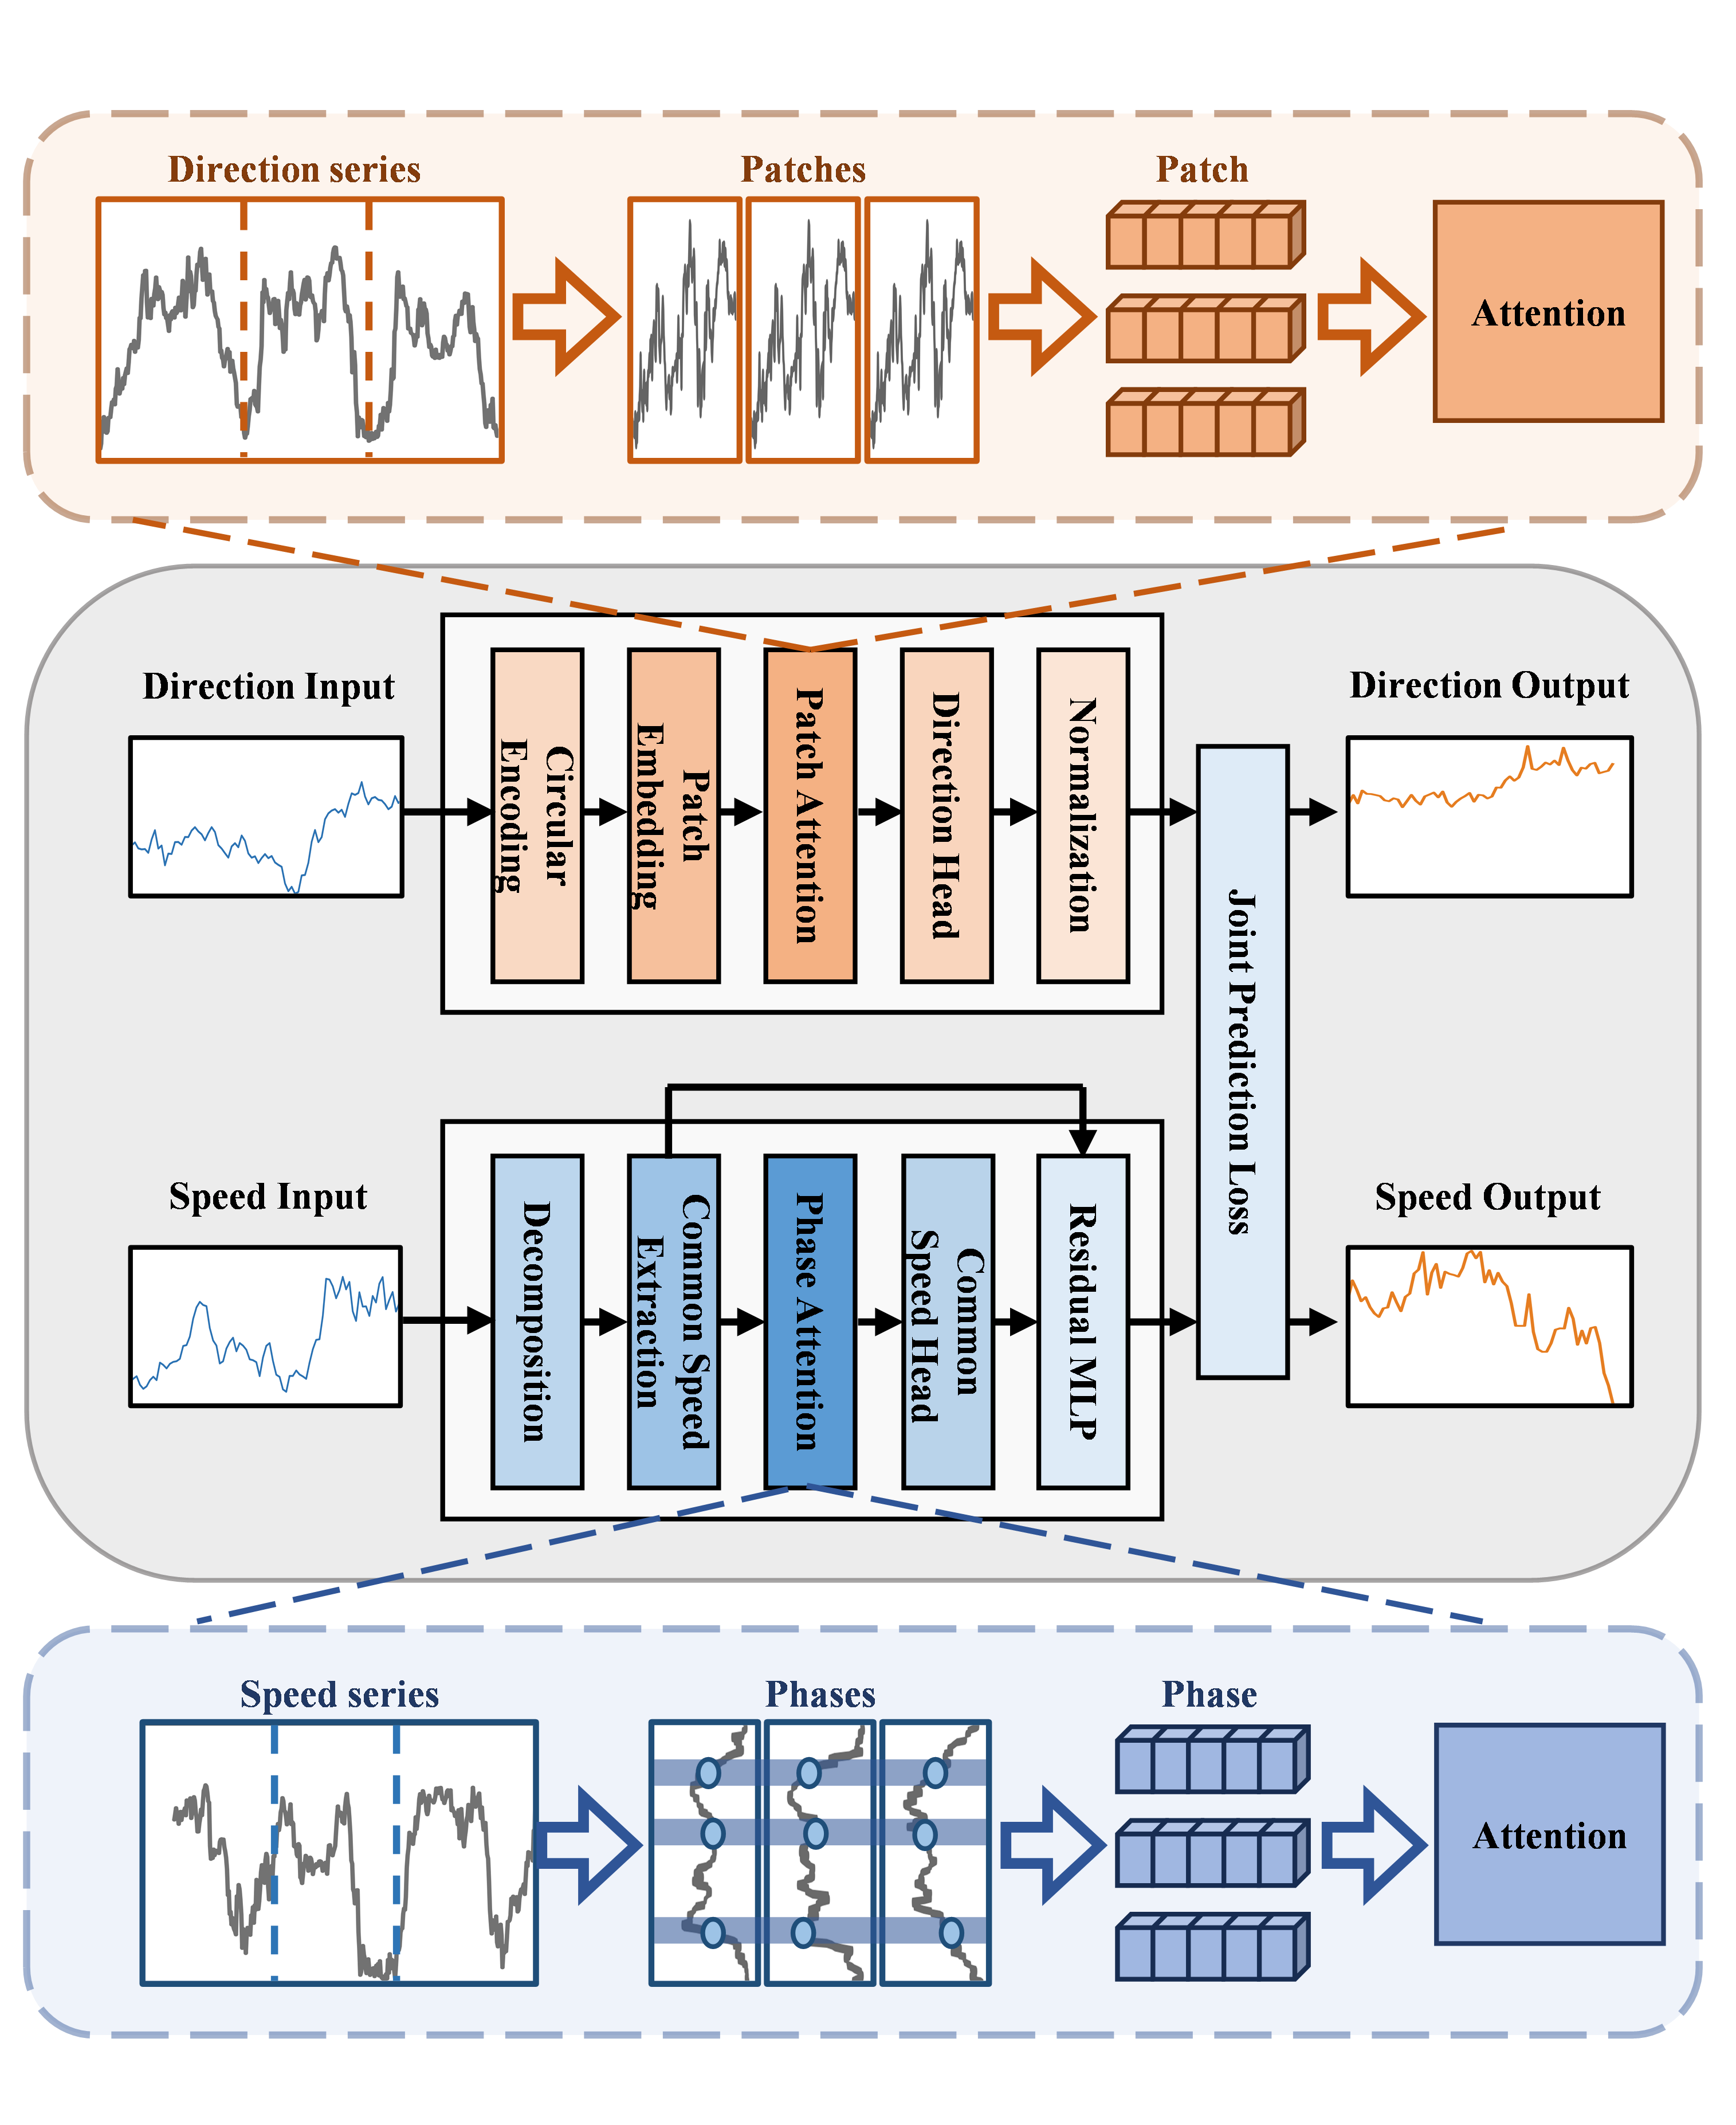
\includegraphics[width=0.5\textwidth]{figures/cscd_architecture.png}
\caption{Overall architecture of WindFormer. The wind speed branch extracts and forecasts common wind speed dynamics with Phase-Attention and restores turbine-level residuals, while the wind direction branch preserves turbine-wise two-dimensional direction sequences through shared Patch-Attention encoding.}
	\label{fig:cscd_architecture}
\end{figure}

\subsection{Overall Model Structure}

The proposed WindFormer is designed around two physical properties of wind farms: wind speeds tend to share common meteorological evolution across turbines, whereas wind directions are recorded as one-dimensional angles and exhibit stronger turbine-specific patterns. As shown in Fig.~\ref{fig:cscd_architecture}, WindFormer contains a wind-speed branch and a wind-direction branch, and the two branches are trained jointly.

Given an input window, the wind-speed branch decomposes the multi-turbine speed field into a common speed component and turbine-level residual components. The common component is encoded by Phase-Attention to capture phase-aligned cross-period evolution, while the residual components are predicted by a shared residual MLP to recover local deviations. The predicted common speed and turbine residuals are then reconstructed into future turbine-wise wind speeds.

The wind-direction branch maps one-dimensional direction angles into two-dimensional sine-cosine unit vectors. For each turbine, the historical two-dimensional direction sequence is partitioned into temporal patches, embedded as patch tokens, and processed by a shared Patch-Attention encoder. A direction prediction head outputs future direction components, which are normalized to unit length before being converted back to angles. This branch preserves turbine-wise directional evolution while sharing temporal parameters across turbines.

The two branches output wind speed and wind direction for the same forecasting horizon. A joint objective combines wind-speed error, direction-vector error, and wind-vector consistency, thereby coupling the two physical quantities during training without forcing them into the same representation space.



\subsection{Learnable Common Wind Speed Extraction}

Let the standardized multi-turbine wind speed be:

\begin{equation}
\tilde{\mathbf{v}}_t = \left[ \tilde{v}_{t,1}, \ldots, \tilde{v}_{t,N} \right].
\end{equation}

The model sets a learnable scalar $a_i$ for each turbine and obtains normalized weights through softmax:

\begin{equation}
\boldsymbol{\alpha} = \operatorname{softmax}(\mathbf{a}), \qquad \sum_{i=1}^{N}\alpha_i=1.
\end{equation}

The common wind speed sequence is defined as:

\begin{equation}
c_t = \sum_{i=1}^{N}\alpha_i\tilde{v}_{t,i}.
\end{equation}

The corresponding wind speed residual for the $i$-th turbine is:

\begin{equation}
r_{t,i} = \tilde{v}_{t,i}-c_t.
\end{equation}

This operation compresses shared wind-farm variations into a common sequence, while turbine-specific deviations are handled by the residual branch.

\subsection{Common Wind Speed Phase-Attention}

\textbf{Candidate period folding.}

Let the common wind speed input sequence be:

\begin{equation}
\mathbf{c}_{1:L} = [c_1, c_2, \ldots, c_L].
\end{equation}

For a candidate period $p$, the model organizes the sequence into multiple local period blocks according to the period position. Let:

\begin{equation}
K_p = \left\lceil\frac{L}{p}\right\rceil,
\end{equation}

then after necessary boundary padding, the sequence can be represented as:

\begin{equation}
\mathbf{C}^{(p)} \in \mathbb{R}^{K_p\times p\times 1}.
\end{equation}

Here, $K_p$ represents the number of period blocks contained in the historical window, and $p$ represents the phase position within each period block. Each period block is flattened into a token:

\begin{equation}
\mathbf{q}^{(p)}_k = \operatorname{Flatten} \left( \mathbf{C}^{(p)}_{k,:,:} \right) \in \mathbb{R}^{p}.
\end{equation}

For multiple candidate periods collected in $\mathcal{P}$, the model organizes short-term temporal patterns at different phase scales.

\textbf{Router-based Phase Attention.}

Each phase token first undergoes linear projection to obtain a $d_m$-dimensional representation, and learnable position encoding is added:

\begin{equation}
\mathbf{e}^{(p)}_k = \operatorname{LN} \left( \mathbf{W}_{\mathrm{in}}^{(p)} \mathbf{q}^{(p)}_k \right) + \mathbf{p}^{(p)}_k.
\end{equation}

To aggregate context across different period blocks, the model introduces $R$ learnable router tokens. Let:

\begin{equation}
\mathbf{R}^{(p)} \in \mathbb{R}^{R\times d_m},
\end{equation}

then the routers first extract global information from the period tokens:

\begin{equation}
\mathbf{C}^{(p)} = \operatorname{Attn} \left( \mathbf{R}^{(p)}, \mathbf{E}^{(p)}, \mathbf{E}^{(p)} \right),
\end{equation}

Subsequently, the period tokens read the cross-period context from the router representations:

\begin{equation}
\widetilde{\mathbf{E}}^{(p)} = \operatorname{Attn} \left( \mathbf{E}^{(p)}, \mathbf{C}^{(p)}, \mathbf{C}^{(p)} \right).
\end{equation}

With residual connections, layer normalization, and feed-forward networks, router tokens summarize cross-period context without full pairwise interaction among all period tokens.

\textbf{Multi-scale common wind speed prediction.}

For each candidate period, the model concatenates the last period token with the average representation of all period tokens:

\begin{equation}
\mathbf{s}^{(p)} = \left[ \widetilde{\mathbf{e}}^{(p)}_{K_p}; \frac{1}{K_p} \sum_{k=1}^{K_p} \widetilde{\mathbf{e}}^{(p)}_k \right].
\end{equation}

Subsequently, the future common wind speed is obtained through the period branch prediction head:

\begin{equation}
\hat{\mathbf{c}}^{(p)} = f_{\mathrm{head}}^{(p)} \left( \mathbf{s}^{(p)} \right) \in \mathbb{R}^{H}.
\end{equation}

The prediction results of different candidate periods are combined by learnable period fusion weights:

\begin{equation}
\hat{\mathbf{c}} = \sum_{p\in\mathcal{P}} \beta_p\hat{\mathbf{c}}^{(p)}, \qquad \beta_p = \frac{\exp(\gamma_p)}{\sum_{q\in\mathcal{P}}\exp(\gamma_q)}.
\end{equation}

Thus, Phase-Attention learns a fusion of multiple short-term candidate scales rather than relying on a single fixed period.

\subsection{Shared Wind Speed Residual Prediction and Reconstruction}

Common wind speed prediction describes shared farm-level variation, while turbine-level residuals recover local dynamics. For the $i$-th turbine, the residual historical sequence is:

\begin{equation}
\mathbf{r}_i = [r_{1,i}, r_{2,i}, \ldots, r_{L,i}].
\end{equation}

The residual branch uses a shared MLP to predict local deviations. Taking the last observed residual $r_{L,i}$ as a reference, the centered sequence is:

\begin{equation}
\widetilde{r}_{t,i} = r_{t,i}-r_{L,i}.
\end{equation}

The shared residual predictor outputs the future residual variation:

\begin{equation}
\Delta\hat{\mathbf{r}}_i = f_{\mathrm{MLP}} \left( \widetilde{\mathbf{r}}_i \right).
\end{equation}

The final residual prediction is:

\begin{equation}
\hat{r}_{h,i} = r_{L,i} + \Delta\hat{r}_{h,i}, \qquad h=1,\ldots,H.
\end{equation}

In the standardized wind speed space, the model uses turbine-level learnable scaling $s_i$ and bias $b_i$ to reconstruct the future wind speed:

\begin{equation}
\hat{\tilde{v}}_{h,i} = s_i\hat{c}_h + b_i + \hat{r}_{h,i}.
\end{equation}

Finally, $\hat{\tilde{v}}_{h,i}$ is unstandardized to obtain the wind speed prediction in the physical space.

\subsection{Wind Direction Independent Patch Transformer}

\textbf{Two-dimensional direction input.}

For the $i$-th turbine, the historical wind direction sequence is represented as:

\begin{equation}
\mathbf{U}_i = \left[ \mathbf{u}_{1,i}, \mathbf{u}_{2,i}, \ldots, \mathbf{u}_{L,i} \right], \qquad \mathbf{u}_{t,i} = [\cos\theta_{t,i}, \sin\theta_{t,i}].
\end{equation}

Accordingly, the direction branch does not extract a common wind direction or construct an additive ``common direction + direction residual'' decomposition. Each turbine direction sequence is maintained as an independent two-dimensional direction input.

\textbf{Temporal patch partitioning.}

For the $L\times 2$ direction sequence of each turbine, a sliding window with length $P$ and step size $S$ constructs temporal patches. The $m$-th patch is:

\begin{equation}
\mathbf{z}_{m,i} = \operatorname{Flatten} \left( \mathbf{U}_{i,(m-1)S+1:(m-1)S+P} \right) \in \mathbb{R}^{2P}.
\end{equation}

The number of generated patches is:

\begin{equation}
M = \left\lfloor \frac{L-P}{S} \right\rfloor+1.
\end{equation}

Each patch contains the sine and cosine components of $P$ time points and is projected to a $d$-dimensional token with positional encoding:

\begin{equation}
\mathbf{e}_{m,i} = \mathbf{W}_{\mathrm{patch}}\mathbf{z}_{m,i} + \mathbf{p}_m.
\end{equation}

This patch representation captures local turning patterns and longer-range directional evolution.

\textbf{Shared Transformer encoding and prediction.}

During direction encoding, each turbine is treated as an independent two-dimensional direction sequence. Turbines share the same patch projection, positional encoding, and Transformer encoder, without token mixing across turbines.

The encoded representation is aggregated using the last patch token and the mean token:

\begin{equation}
\mathbf{h}_i = \left[ \mathbf{e}_{M,i}^{\mathrm{enc}}; \frac{1}{M} \sum_{m=1}^{M} \mathbf{e}_{m,i}^{\mathrm{enc}} \right].
\end{equation}

The prediction head maps $\mathbf{h}_i$ to the two-dimensional direction components for the future $H$ time steps:

\begin{equation}
\hat{\mathbf{U}}_i = f_{\theta}(\mathbf{h}_i) \in \mathbb{R}^{H\times 2}.
\end{equation}

The predicted vectors are L2-normalized before angle recovery:

\begin{equation}
\hat{\mathbf{u}}_{h,i} = \frac{\hat{\mathbf{u}}_{h,i}}{\|\hat{\mathbf{u}}_{h,i}\|_2+\epsilon}.
\end{equation}

Then $\operatorname{atan2}$ recovers the wind direction angle.

\subsection{Joint Loss Function}

\textbf{Wind speed loss.}

Wind speed prediction uses Mean Squared Error in the standardized space:

\begin{equation}
\mathcal{L}_{v} = \operatorname{MSE} \left( \hat{\tilde{\mathbf{V}}}, \tilde{\mathbf{V}} \right).
\end{equation}

\textbf{Direction-vector loss.}

For the predicted direction and true direction, unit vectors are obtained respectively:

\begin{equation}
\hat{\mathbf{u}}_{t,i} = [\hat{u}^{\cos}_{t,i}, \hat{u}^{\sin}_{t,i}], \qquad \mathbf{u}_{t,i} = [u^{\cos}_{t,i}, u^{\sin}_{t,i}].
\end{equation}

The direction error is defined using two-dimensional vector consistency:

\begin{equation}
\ell_{\theta,t,i} = 1 - \hat{\mathbf{u}}_{t,i}^{\mathsf{T}} \mathbf{u}_{t,i}.
\end{equation}

At low wind speeds, wind direction observations are more susceptible to noise; therefore, a reliability weight based on physical wind speed is used:

\begin{equation}
w_{t,i} = \operatorname{clip} \left( \frac{v_{t,i}}{v_0}, 0, 1 \right),
\end{equation}

where $v_0$ is the wind-speed threshold controlling the reliability weight. The weighted direction loss is:

\begin{equation}
\mathcal{L}_{\theta} = \frac{\sum_{t,i}w_{t,i}\ell_{\theta,t,i}}{\sum_{t,i}w_{t,i}+\epsilon}.
\end{equation}

This loss constrains the angle between predicted and true two-dimensional direction vectors and avoids boundary errors from scalar-angle regression.

\textbf{Wind vector consistency loss.}

To constrain speed-direction consistency, physical wind speed is combined with the unit direction vector:

\begin{equation}
\mathbf{q}_{t,i} = v_{t,i} \left[ \cos\theta_{t,i}, \sin\theta_{t,i} \right],
\end{equation}

After scale normalization, predicted and true wind vectors are compared by Smooth L1 loss:

\begin{equation}
\mathcal{L}_{q} = \operatorname{SmoothL1} \left( \frac{\hat{\mathbf{q}}}{\bar{\sigma}_v}, \frac{\mathbf{q}}{\bar{\sigma}_v} \right),
\end{equation}

where $\bar{\sigma}_v$ is the average of the wind speed standard deviations of all turbines.

\textbf{Overall objective.}

The final training objective is:

\begin{equation}
\mathcal{L} = \lambda_v\mathcal{L}_{v} + \lambda_\theta\mathcal{L}_{\theta} + \lambda_q\mathcal{L}_{q}.
\end{equation}

The coefficients balance the wind-speed objective, the direction-vector objective, and the auxiliary wind-vector consistency constraint.

\section{Experiments}
\label{sec:experiments}

\begin{figure}[!t]
	\centering
	
\includegraphics[width=0.42\textwidth]{figures/data.png}
	\caption{Geographical visualization of the two wind farm datasets used in the experiments.}
	\label{fig:dataset_geography}
\end{figure}

\begin{table*}[!t]
	\caption{Detailed full-sample forecasting performance on the Penmanshiel dataset under the noise-free setting. Lower values indicate better performance.}
	\label{tab:main_penmanshiel}
	\centering
	\scriptsize
	\setlength{\tabcolsep}{5pt}
	\renewcommand{\arraystretch}{1.04}
	\begin{adjustbox}{max width=\textwidth}
		\begin{tabular}{llcccccccc}
			\toprule
			Metric & Horizon & WindFormer & MST-Net & TimeMixer++ & iTransformer & PatchTST & TimesNet & GLPT & DLinear \\
			\midrule
			\multirow{3}{*}{Speed MAE} & 6 & \textbf{0.7142} & 0.7978 & 0.9229 & 0.9272 & 0.9189 & 0.9210 & 0.9318 & 0.9263 \\
			& 12 & \textbf{0.8812} & 0.9879 & 1.1421 & 1.1491 & 1.1347 & 1.1406 & 1.1543 & 1.1473 \\
			& 18 & \textbf{1.0103} & 1.1249 & 1.2994 & 1.3081 & 1.2891 & 1.2976 & 1.3138 & 1.3061 \\
			\midrule
			\multirow{3}{*}{Speed RMSE} & 6 & \textbf{1.1497} & 1.2162 & 1.3053 & 1.3118 & 1.2987 & 1.3033 & 1.3174 & 1.3108 \\
			& 12 & \textbf{1.4211} & 1.5538 & 1.6162 & 1.6247 & 1.6054 & 1.6142 & 1.6325 & 1.6224 \\
			& 18 & \textbf{1.6216} & 1.7599 & 1.8367 & 1.8477 & 1.8263 & 1.8348 & 1.8553 & 1.8447 \\
			\midrule
			\multirow{3}{*}{Direction MAE} & 6 & \textbf{0.1456} & 0.1637 & 0.1898 & 0.1911 & 0.1884 & 0.1894 & 0.1926 & 0.1939 \\
			& 12 & \textbf{0.1881} & 0.2113 & 0.2439 & 0.2460 & 0.2403 & 0.2434 & 0.2483 & 0.2497 \\
			& 18 & \textbf{0.2204} & 0.2471 & 0.2847 & 0.2872 & 0.2807 & 0.2840 & 0.2899 & 0.2913 \\
			\midrule
			\multirow{3}{*}{Direction RMSE} & 6 & \textbf{0.2914} & 0.3092 & 0.3314 & 0.3341 & 0.3294 & 0.3320 & 0.3354 & 0.3375 \\
			& 12 & \textbf{0.3686} & 0.3905 & 0.4176 & 0.4213 & 0.4146 & 0.4184 & 0.4237 & 0.4260 \\
			& 18 & \textbf{0.4244} & 0.4599 & 0.4796 & 0.4843 & 0.4761 & 0.4807 & 0.4870 & 0.4906 \\
			\bottomrule
		\end{tabular}
	\end{adjustbox}
\end{table*}

\subsection{Experimental Setup}
\label{subsec:experimental_setup}

We evaluate the model on two SCADA-based wind farm datasets with distinct spatial layouts and wind regimes: Shanxi with 24 turbines and Penmanshiel with 14 turbines. Both datasets are sampled at 10-min intervals and preprocessed following the protocol in Section~\ref{sec:data_preprocessing_task}. Unless otherwise specified, the input window is 288 steps, corresponding to 48 h of history, and the forecasting horizons are 6, 12, and 18 steps.



WindFormer is compared with MST-Net, PatchTST, TimeMixer++, GLPT, DLinear, TimesNet, and iTransformer. MAE and RMSE are reported for wind speed (m/s) and wind direction (rad). Beyond the full-sample benchmark, robustness and sparse-deployment generalization are further evaluated.

\subsection{Standard Forecasting Evaluation}
\label{subsec:standard_forecasting}

The standard setting trains and tests on the full turbine set without artificial perturbation.



\begin{table*}[!t]
\caption{Detailed full-sample forecasting performance on the Shanxi dataset under the noise-free setting. Lower values indicate better performance.}
\label{tab:main_shanxi}
\centering
\scriptsize
\setlength{\tabcolsep}{5pt}
\renewcommand{\arraystretch}{1.04}
\begin{adjustbox}{max width=\textwidth}
\begin{tabular}{llcccccccc}
\toprule
			Metric & Horizon & WindFormer & MST-Net & TimeMixer++ & iTransformer & PatchTST & TimesNet & GLPT & DLinear \\
\midrule
\multirow{3}{*}{Speed MAE} & 6 & \textbf{0.6367} & 0.7062 & 0.8192 & 0.8222 & 0.8165 & 0.8274 & 0.8270 & 0.8217 \\
 & 12 & \textbf{0.8025} & 0.8939 & 1.0343 & 1.0395 & 1.0309 & 1.0452 & 1.0447 & 1.0379 \\
 & 18 & \textbf{0.9309} & 1.0337 & 1.1970 & 1.2024 & 1.1953 & 1.2098 & 1.2094 & 1.2013 \\
\midrule
\multirow{3}{*}{Speed RMSE} & 6 & \textbf{0.9884} & 1.0377 & 1.1203 & 1.1248 & 1.1172 & 1.1320 & 1.1311 & 1.1242 \\
 & 12 & \textbf{1.2374} & 1.3033 & 1.4035 & 1.4097 & 1.3986 & 1.4178 & 1.4167 & 1.4078 \\
 & 18 & \textbf{1.4116} & 1.4862 & 1.6002 & 1.6073 & 1.5987 & 1.6172 & 1.6161 & 1.6059 \\
\midrule
\multirow{3}{*}{Direction MAE} & 6 & \textbf{0.2717} & 0.2984 & 0.3460 & 0.3478 & 0.3445 & 0.3507 & 0.3500 & 0.3516 \\
 & 12 & \textbf{0.3441} & 0.3806 & 0.4403 & 0.4426 & 0.4384 & 0.4465 & 0.4459 & 0.4476 \\
 & 18 & \textbf{0.4019} & 0.4437 & 0.5130 & 0.5160 & 0.5115 & 0.5206 & 0.5199 & 0.5223 \\
\midrule
\multirow{3}{*}{Direction RMSE} & 6 & \textbf{0.5530} & 0.5778 & 0.6225 & 0.6269 & 0.6210 & 0.6283 & 0.6273 & 0.6300 \\
 & 12 & \textbf{0.6525} & 0.7041 & 0.7356 & 0.7409 & 0.7342 & 0.7454 & 0.7440 & 0.7471 \\
 & 18 & \textbf{0.7275} & 0.7831 & 0.8196 & 0.8255 & 0.8184 & 0.8295 & 0.8285 & 0.8324 \\
\bottomrule
\end{tabular}
\end{adjustbox}
\end{table*}

\begin{figure}[!t]
\centering
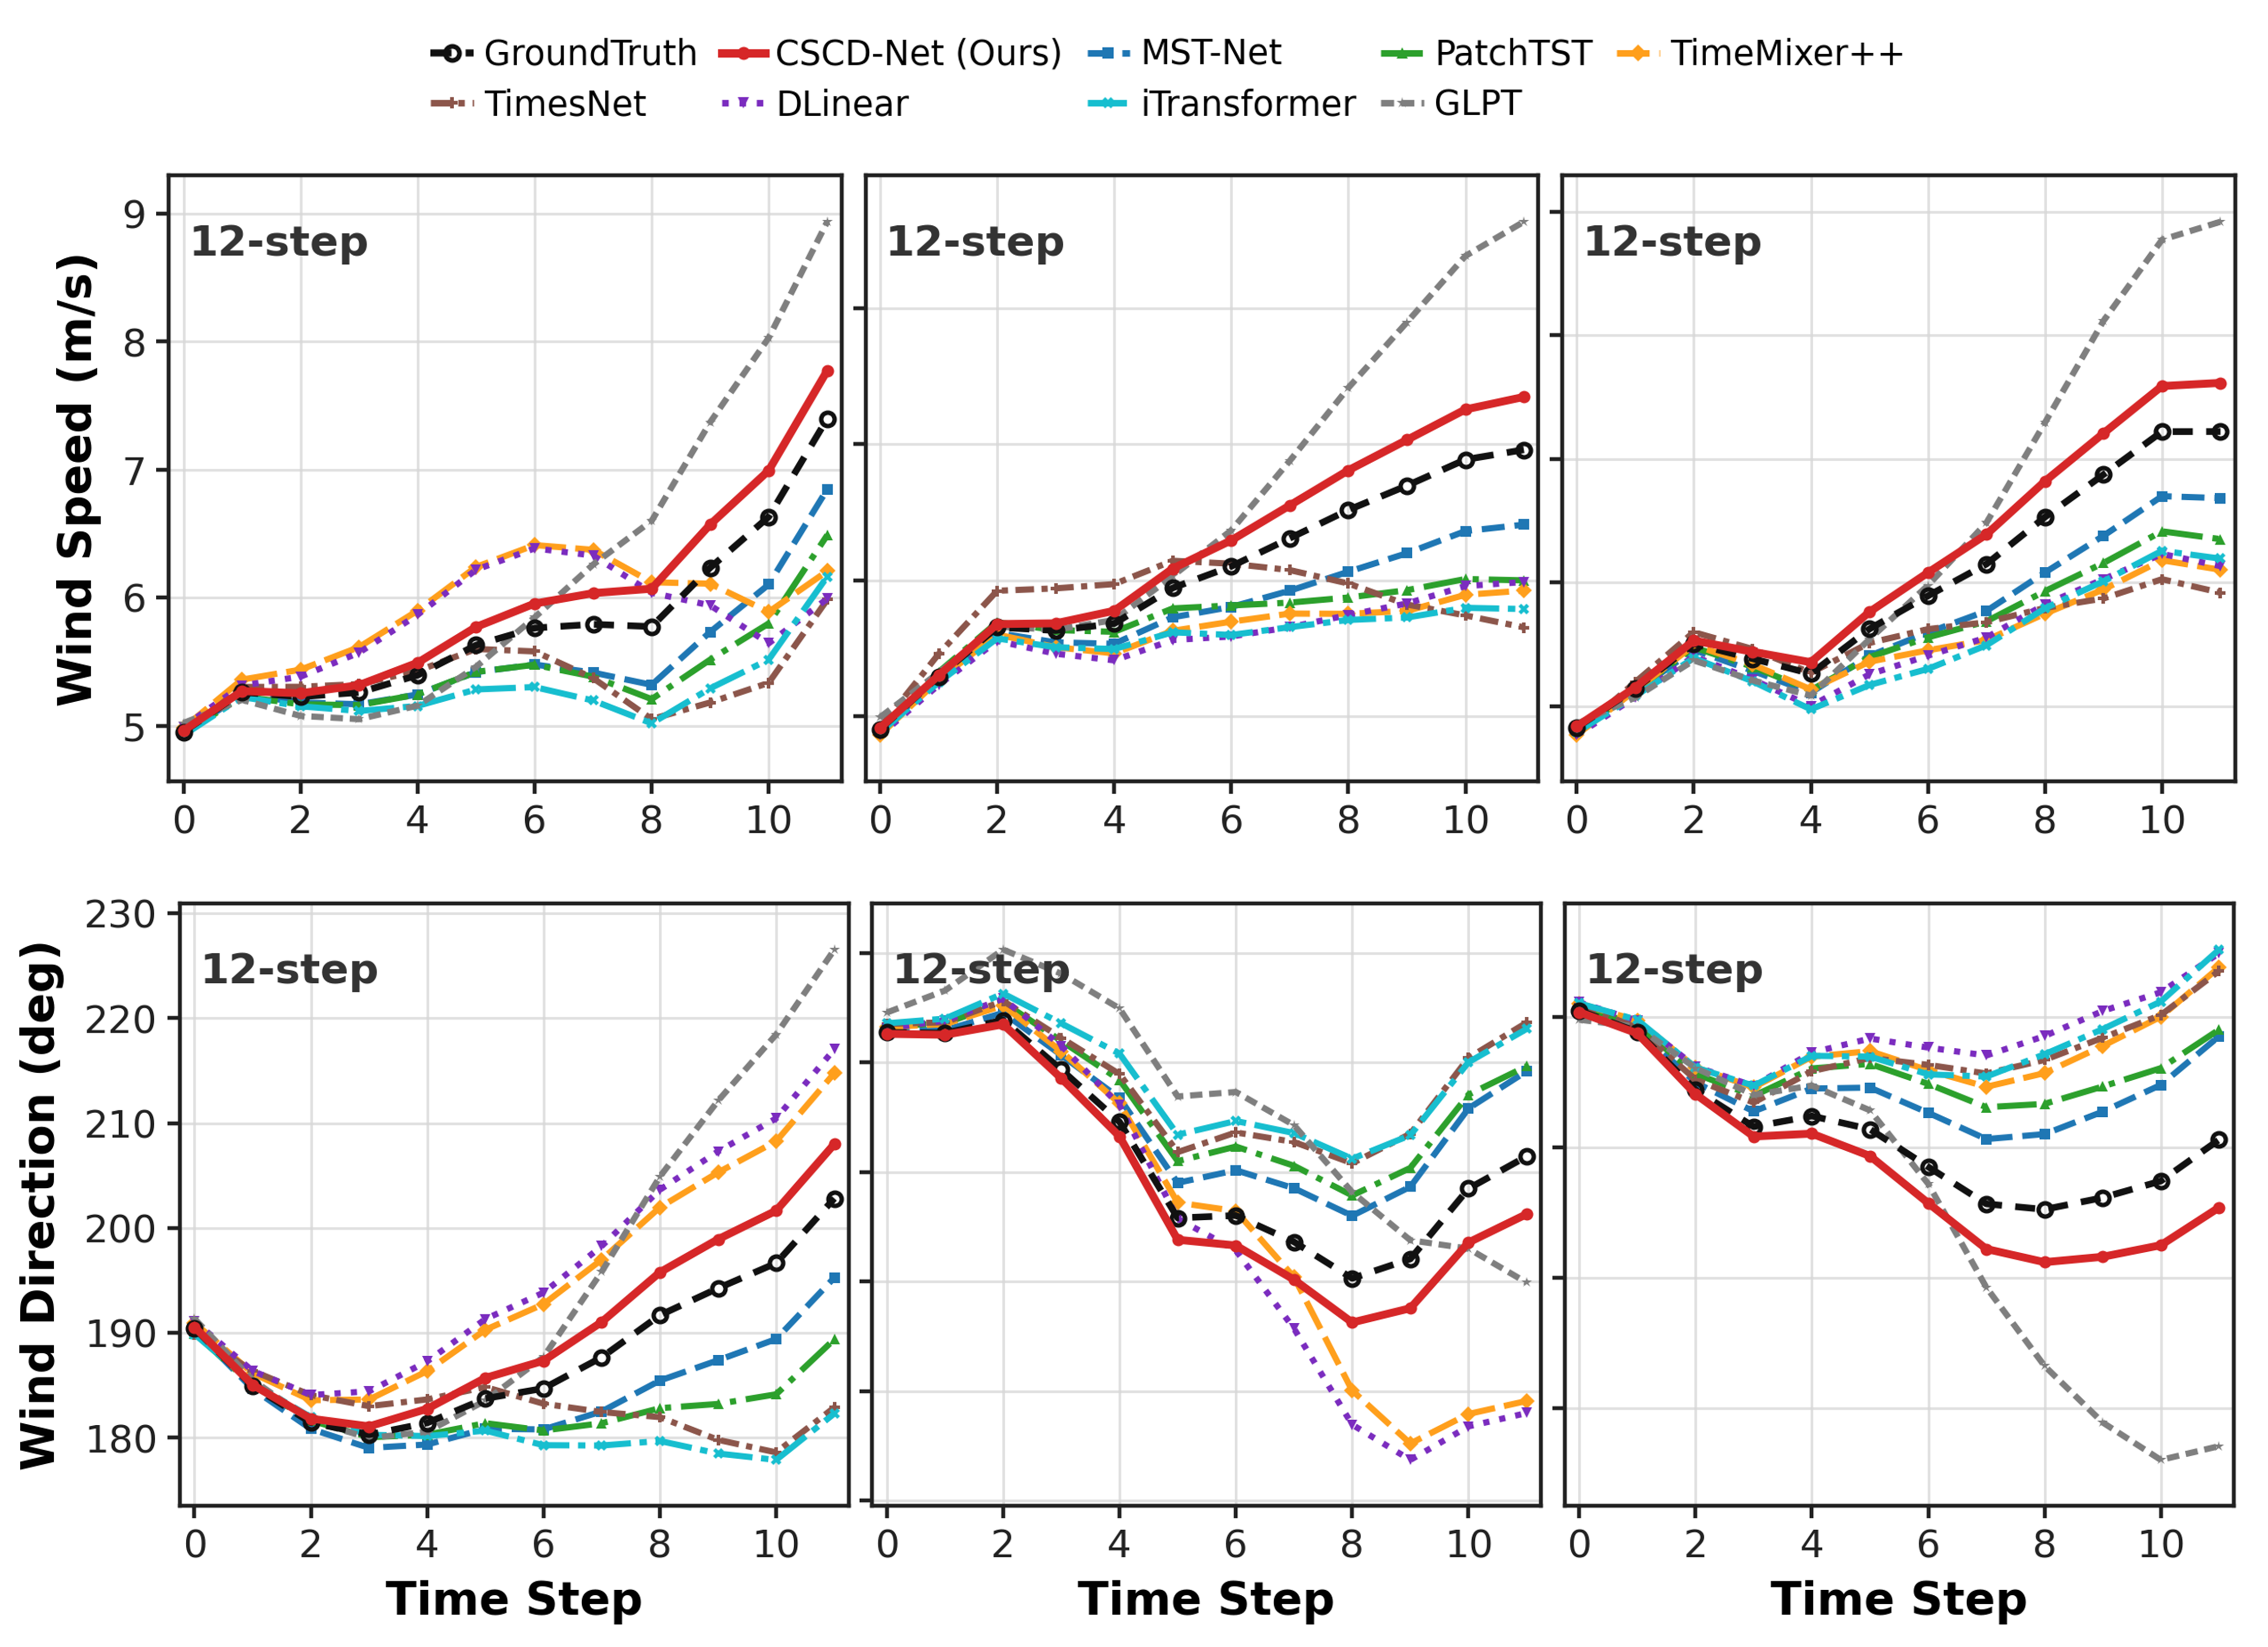
\includegraphics[width=0.48\textwidth]{figures/result.png}
\caption{Representative 12-step full-sample prediction examples for wind speed and wind direction.}
\label{fig:prediction_examples}
\end{figure}

Tables~\ref{tab:main_penmanshiel} and \ref{tab:main_shanxi} show that WindFormer achieves the best wind speed and wind direction accuracy across all horizons on both datasets.

\begin{table}[!t]
\caption{Computational efficiency comparison at the 12-step forecasting horizon.}
\label{tab:efficiency}
\centering
\scriptsize
\setlength{\tabcolsep}{2.0pt}
\renewcommand{\arraystretch}{1.04}
\begin{adjustbox}{max width=\columnwidth}
\begin{tabular}{@{}lccccc@{}}
\toprule
Metric & WindFormer & MSGNet & PatchTST & iTransformer & TimeMixer++ \\
\midrule
Parameters & 36,512 & 26,680,000 & 140,492 & 124,428 & 388,332 \\
Train time (s) & 143.78 & 14356.30 & 315.32 & 57.80 & 109.55 \\
Peak GPU (MB) & 74.83 & 4532.1 & 3158.9 & 109.1 & 308.9 \\
\bottomrule
\end{tabular}
\end{adjustbox}
\end{table}

Table~\ref{tab:efficiency} shows that WindFormer achieves competitive efficiency with 36,512 parameters and 74.83 MB peak GPU memory.

\subsection{Robustness Under Perturbation}
\label{subsec:robustness}

Two robustness experiments are designed: \emph{Sensor Perturbation Robustness} and \emph{Extreme Volatility Stress Test}. For sensor perturbation, let $\theta_{i,t}$ denote the wind direction of turbine $i$ at time $t$, and let $\mathcal{W}(\cdot)$ wrap angles to the valid range. Only the wind-direction channel in the training inputs is corrupted as
\begin{equation}
\tilde{\theta}_{i,t}^{(\sigma)}=\mathcal{W}\left(\theta_{i,t}+\epsilon_{i,t}^{(\sigma)}\right),\quad
\epsilon_{i,t}^{(\sigma)}\sim\mathcal{N}(0,\sigma^2),
\label{eq:sensor_noise}
\end{equation}
where $\sigma\in\{0.1,0.2,0.3\}$ rad. Test inputs and labels remain unchanged, and all models are retrained at each noise level.

\begin{figure}[!t]
\centering
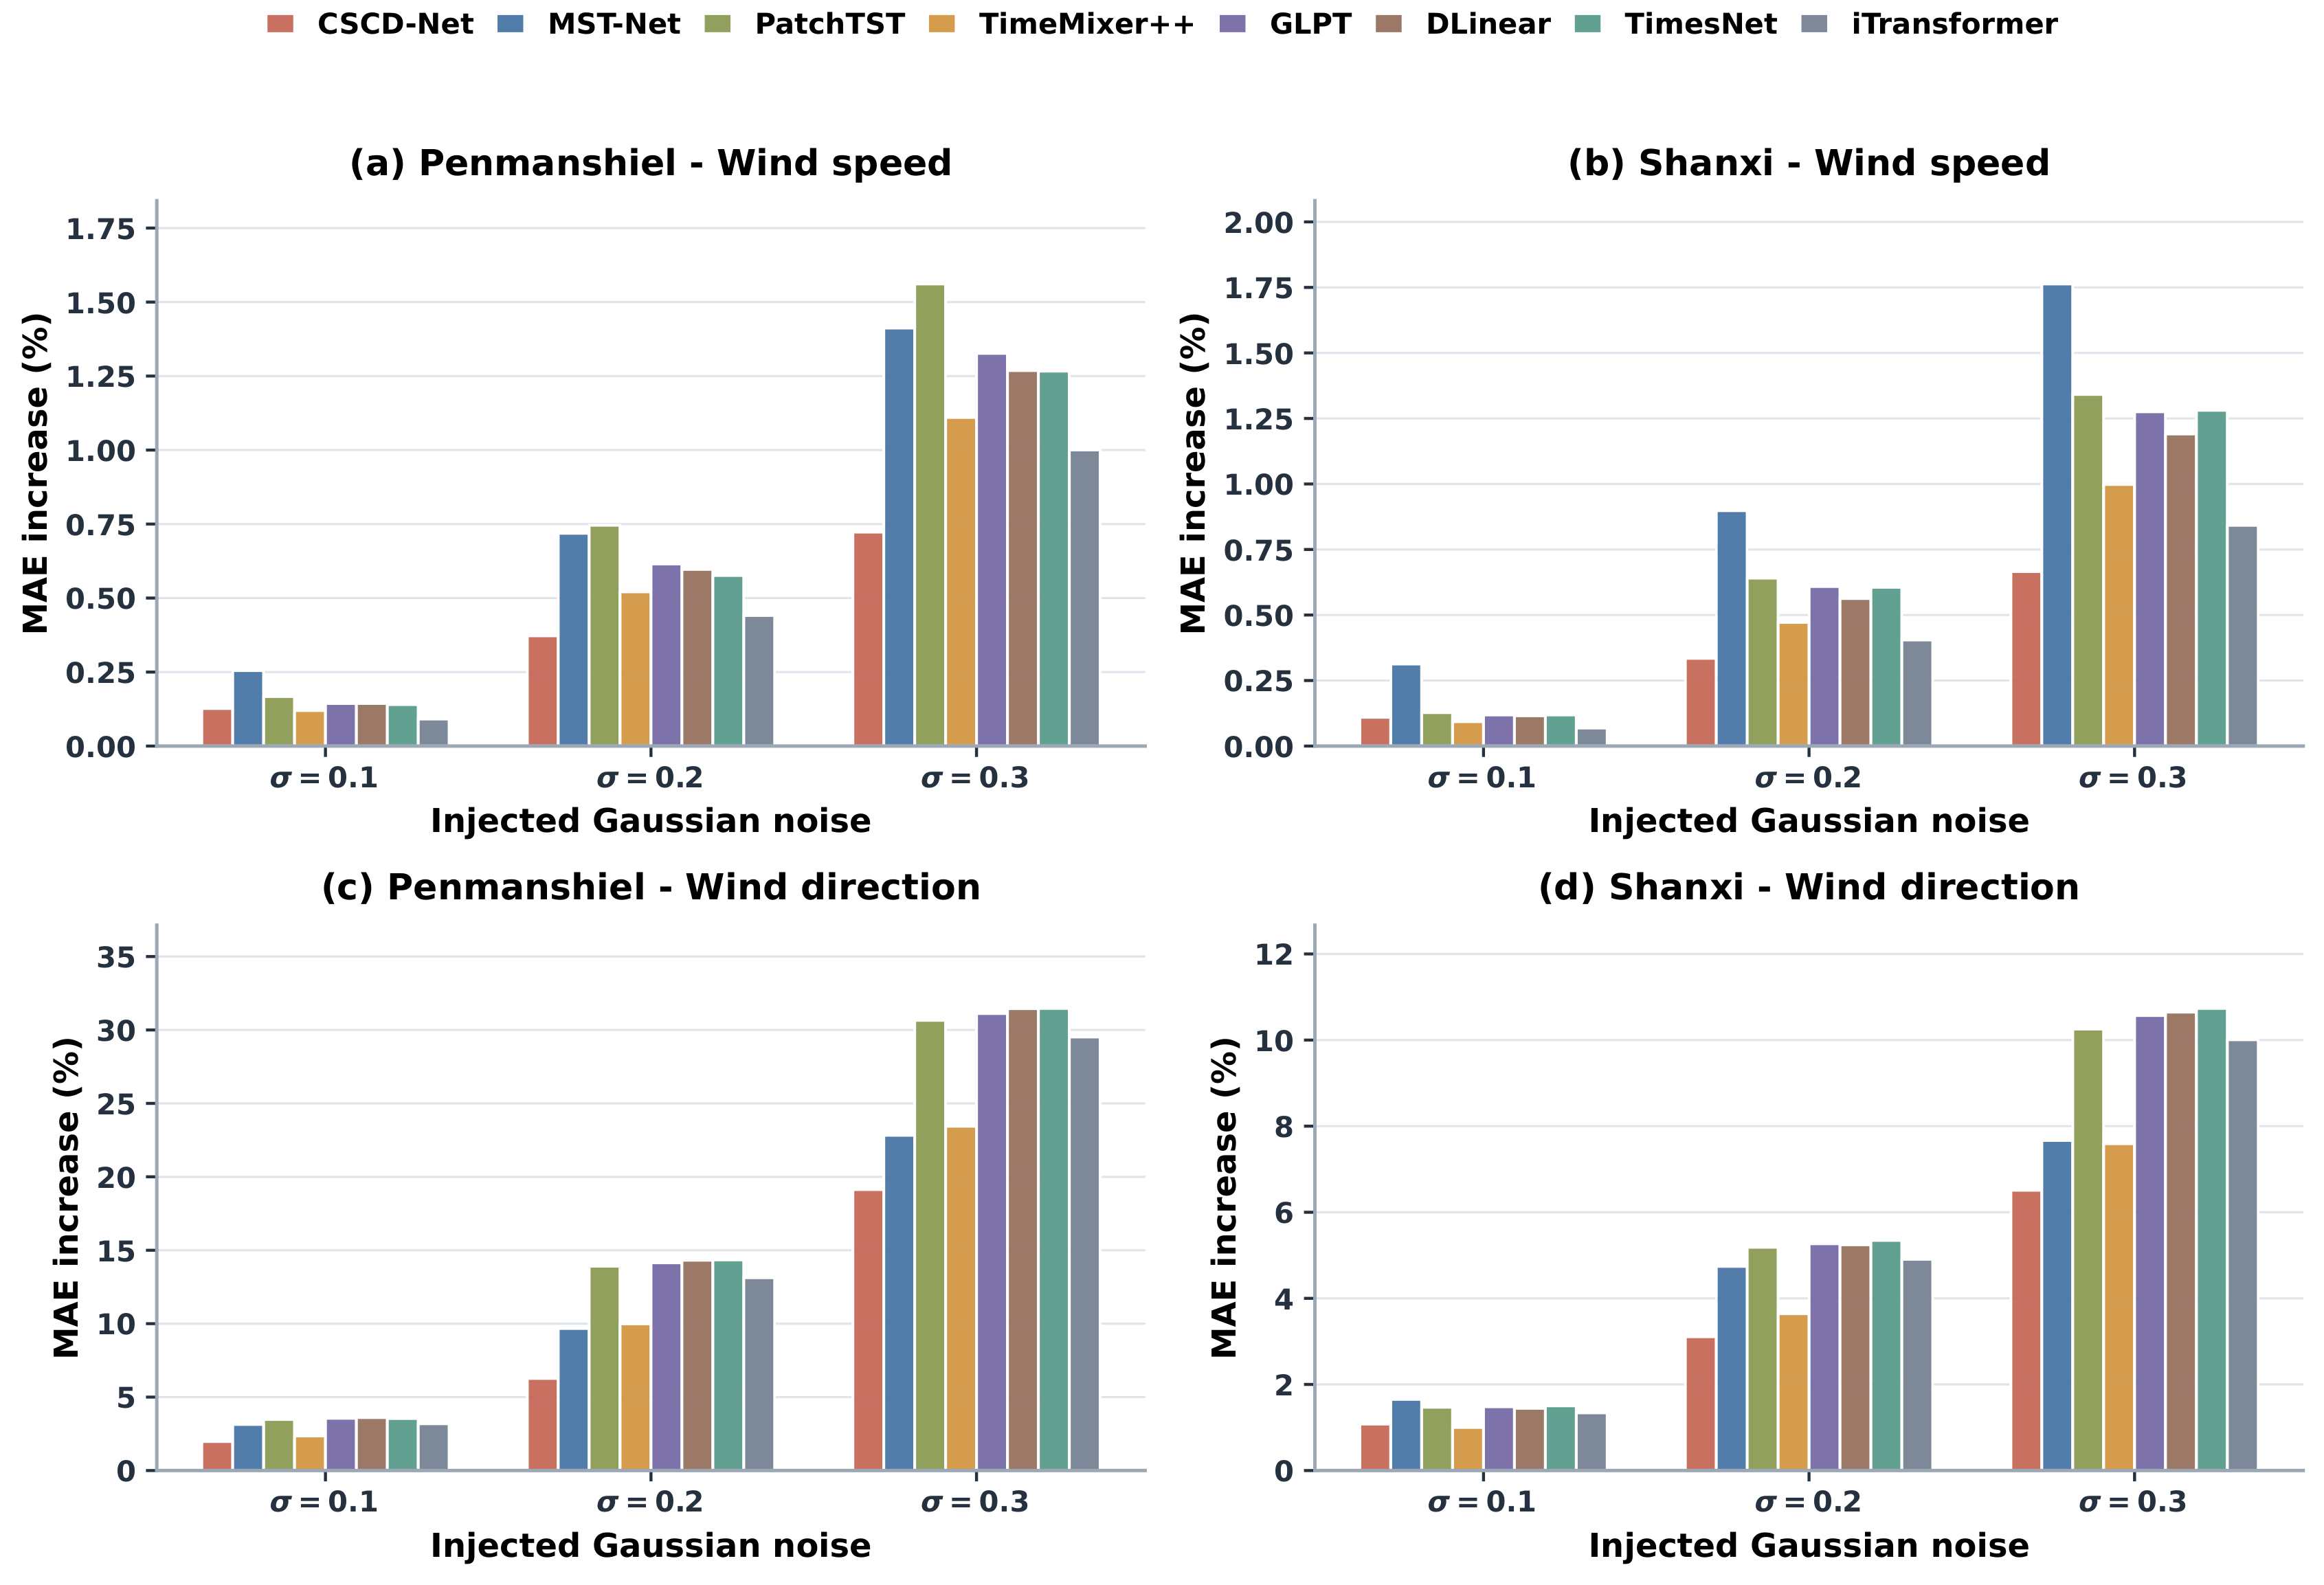
\includegraphics[width=0.48\textwidth]{figures/supp_sensor_robustness.png}
\caption{Sensor Perturbation Robustness. The comparison covers all models, both wind speed and wind direction, and both datasets. Each subplot uses its own vertical scale to preserve dataset-specific variation.}
\label{fig:sensor_perturbation}
\end{figure}

The second experiment evaluates gust-like transient fluctuations through an EVT-inspired residual stratification scheme \cite{Pickands1975StatisticalInferenceUsingExtremeOrderStatistics,Cleveland1990STLSeasonalTrendDecomposition}. For a target series $y_t$, seasonal-trend decomposition using LOESS gives
\begin{equation}
y_t=T_t+S_t+R_t,
\end{equation}
where $T_t$, $S_t$, and $R_t$ denote the trend, seasonal, and residual terms, respectively. The extreme threshold is estimated only from the training split:
\begin{equation}
u=Q_{0.99}\left(\{|R_t|:t\in\mathcal{T}_{\mathrm{train}}\}\right),
\end{equation}
where $Q_{0.99}(\cdot)$ is the 99th percentile. A time step is identified as an extreme event when
\begin{equation}
I_t=\mathbb{I}(|R_t|>u).
\end{equation}
Given an input window of length $L=288$ ending at time $t$, the volatility severity of the corresponding forecasting sample is quantified by
\begin{equation}
N_{\mathrm{extreme}}(t)=\sum_{\tau=t-L+1}^{t}I_{\tau}.
\end{equation}
Test samples are binned by $N_{\mathrm{extreme}}(t)$ and evaluated with the trained model held fixed.

\begin{figure}[!t]
\centering
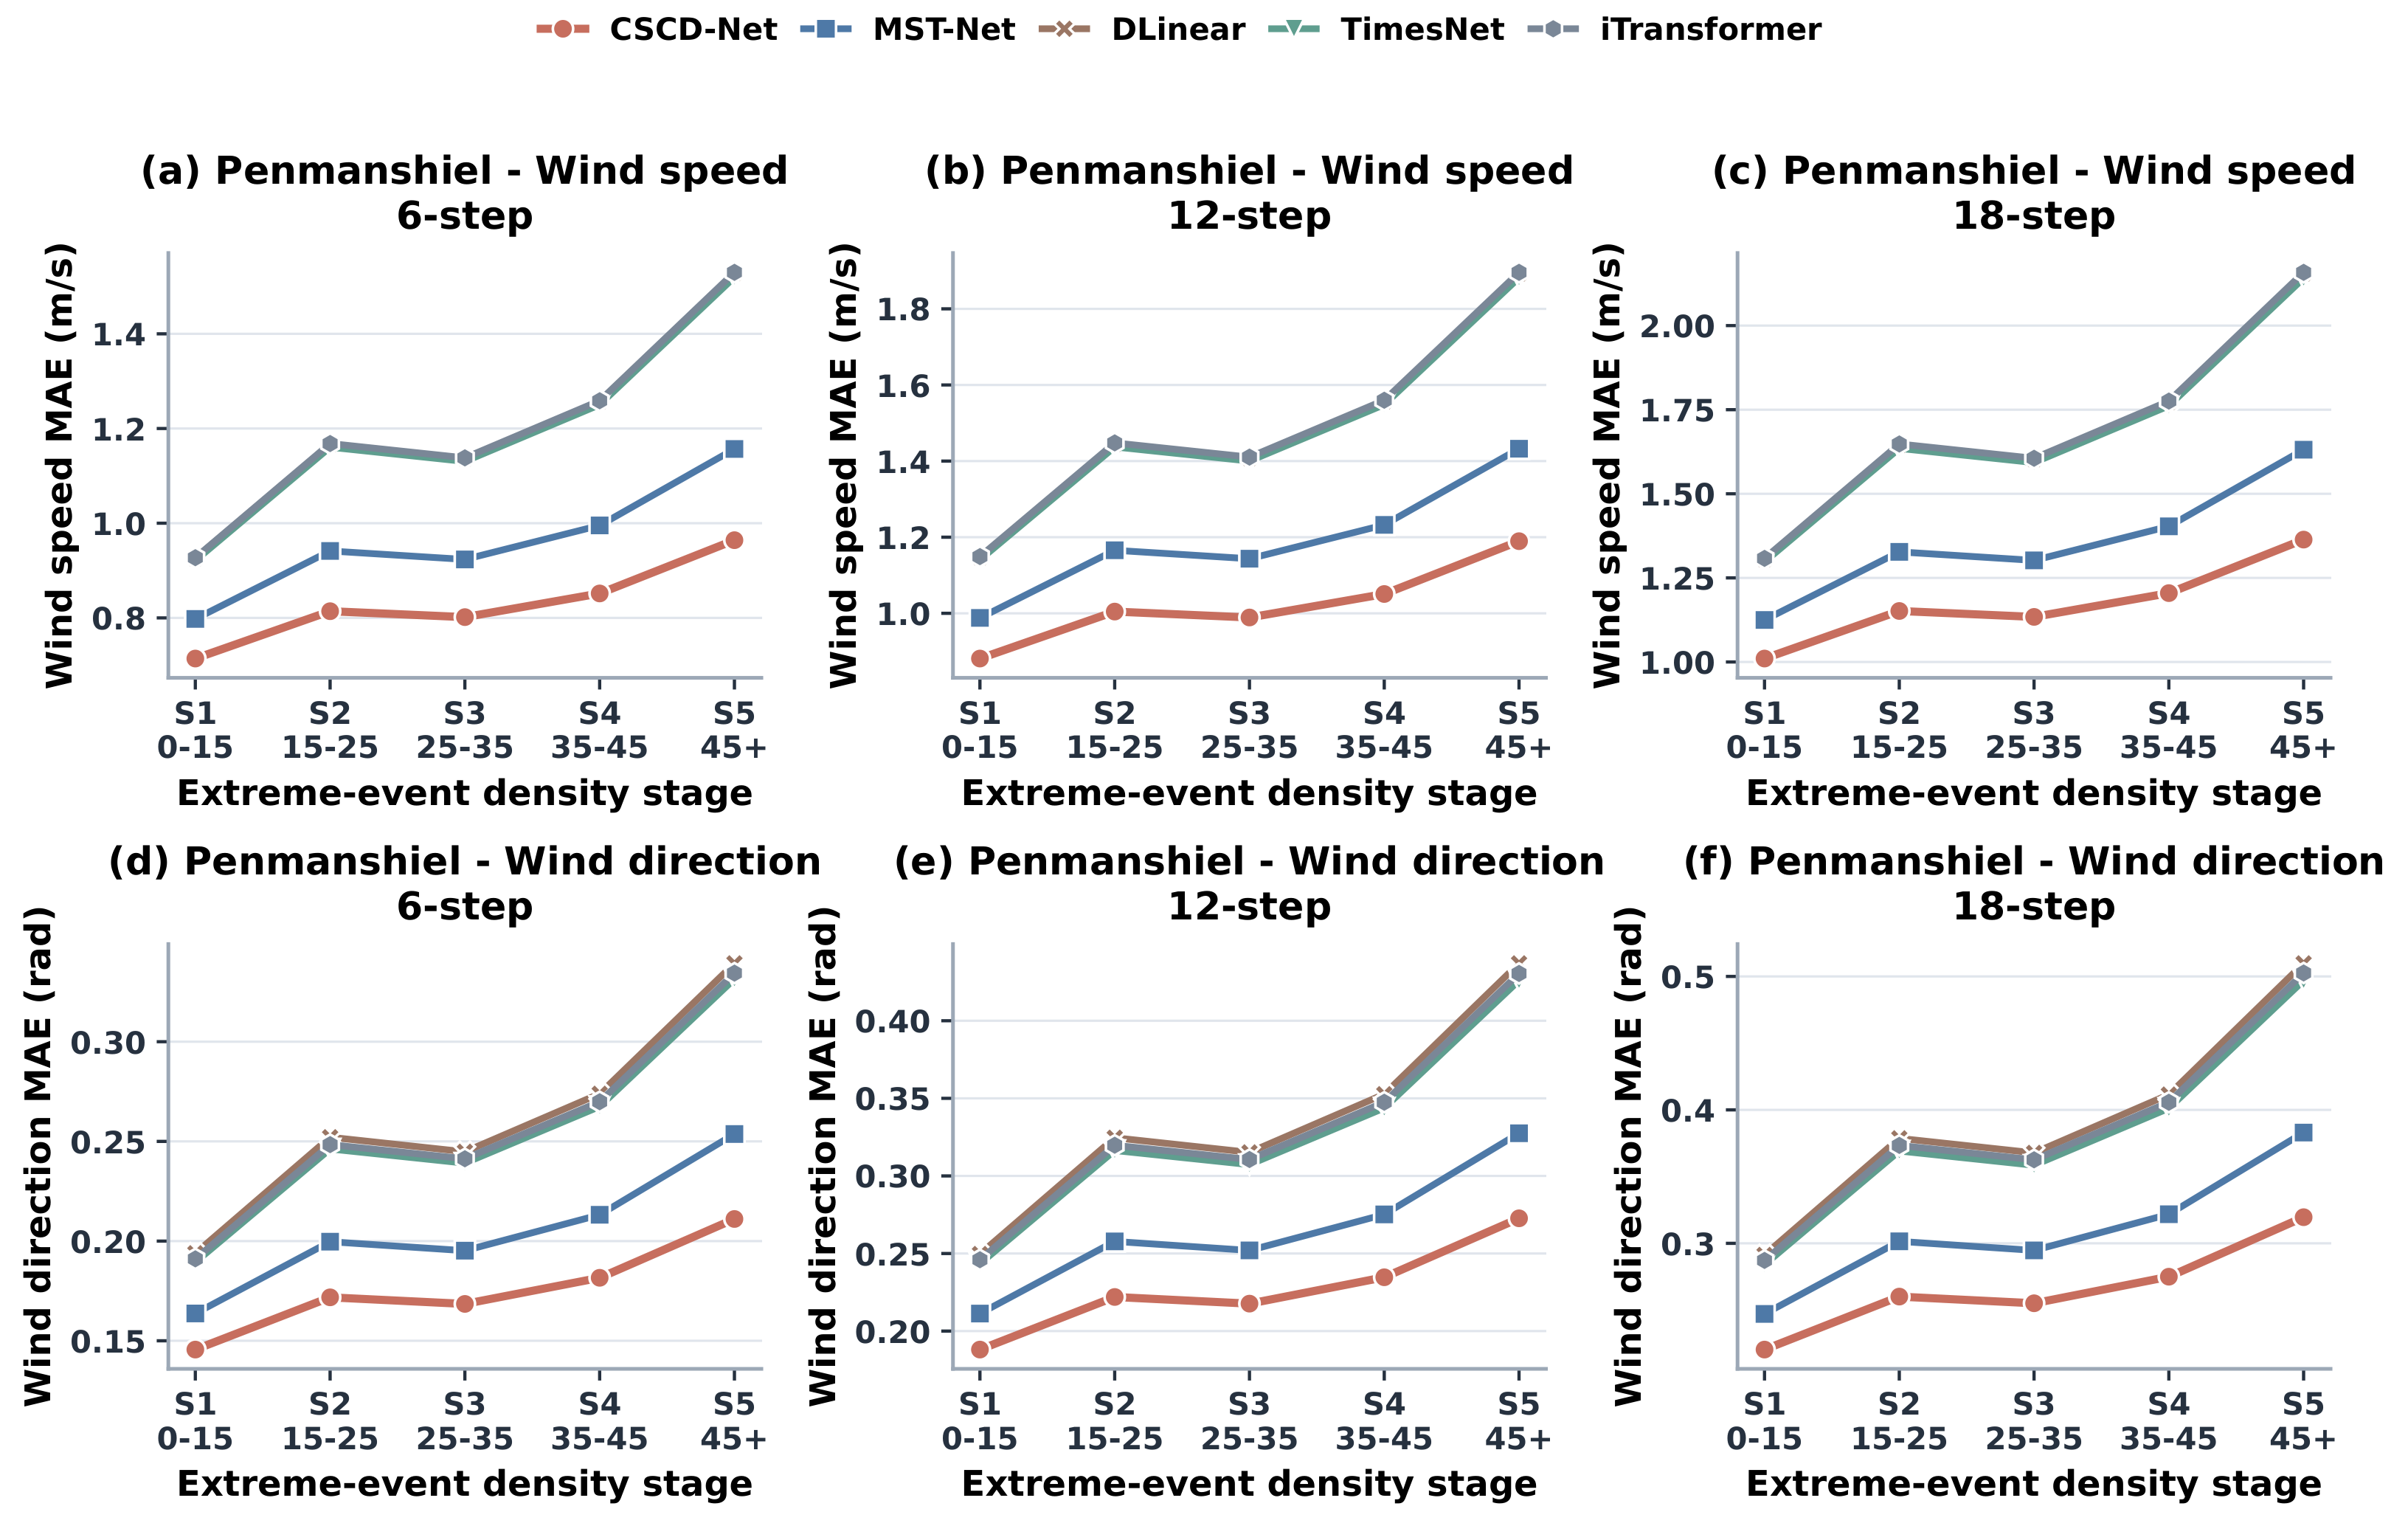
\includegraphics[width=0.48\textwidth]{figures/supp_extreme_stress.png}
\caption{Extreme Volatility Stress Test on the Penmanshiel dataset. The figure reports wind speed and wind direction errors under increasing values of $N_{\mathrm{extreme}}$.}
\label{fig:extreme_stress}
\end{figure}

Figs.~\ref{fig:sensor_perturbation} and \ref{fig:extreme_stress} show that WindFormer yields the smallest degradation under both sensor noise and increasing extreme residual severity.

\subsection{Sparse Deployment Zero-Shot Evaluation}
\label{subsec:zero_shot}

We conduct the \emph{Sparse Deployment Zero-Shot Evaluation} on Penmanshiel. Let $\mathcal{V}$ denote all turbines and $\mathcal{S}_k\subset\mathcal{V}$ the four turbines randomly selected in trial $k$. The remaining turbines
\begin{equation}
\mathcal{U}_k=\mathcal{V}\setminus\mathcal{S}_k
\end{equation}
are treated as unseen zero-shot targets. For a model $f_{\phi}$, $\phi$ is trained only on $\mathcal{D}_{\mathrm{train}}(\mathcal{S}_k)$ and evaluated on $\mathcal{D}_{\mathrm{test}}(\mathcal{U}_k)$. The reported error is averaged over three independent trials:
\begin{equation}
\mathrm{Err}_{\mathrm{ZS}}=\frac{1}{3}\sum_{k=1}^{3}\mathrm{Err}\left(f_{\phi_k},\mathcal{D}_{\mathrm{test}}(\mathcal{U}_k)\right).
\end{equation}
Three conditions are compared: full-sample training, zero-shot transfer, and zero-shot transfer with 0.3-rad angular noise.

\begin{figure}[!t]
\centering
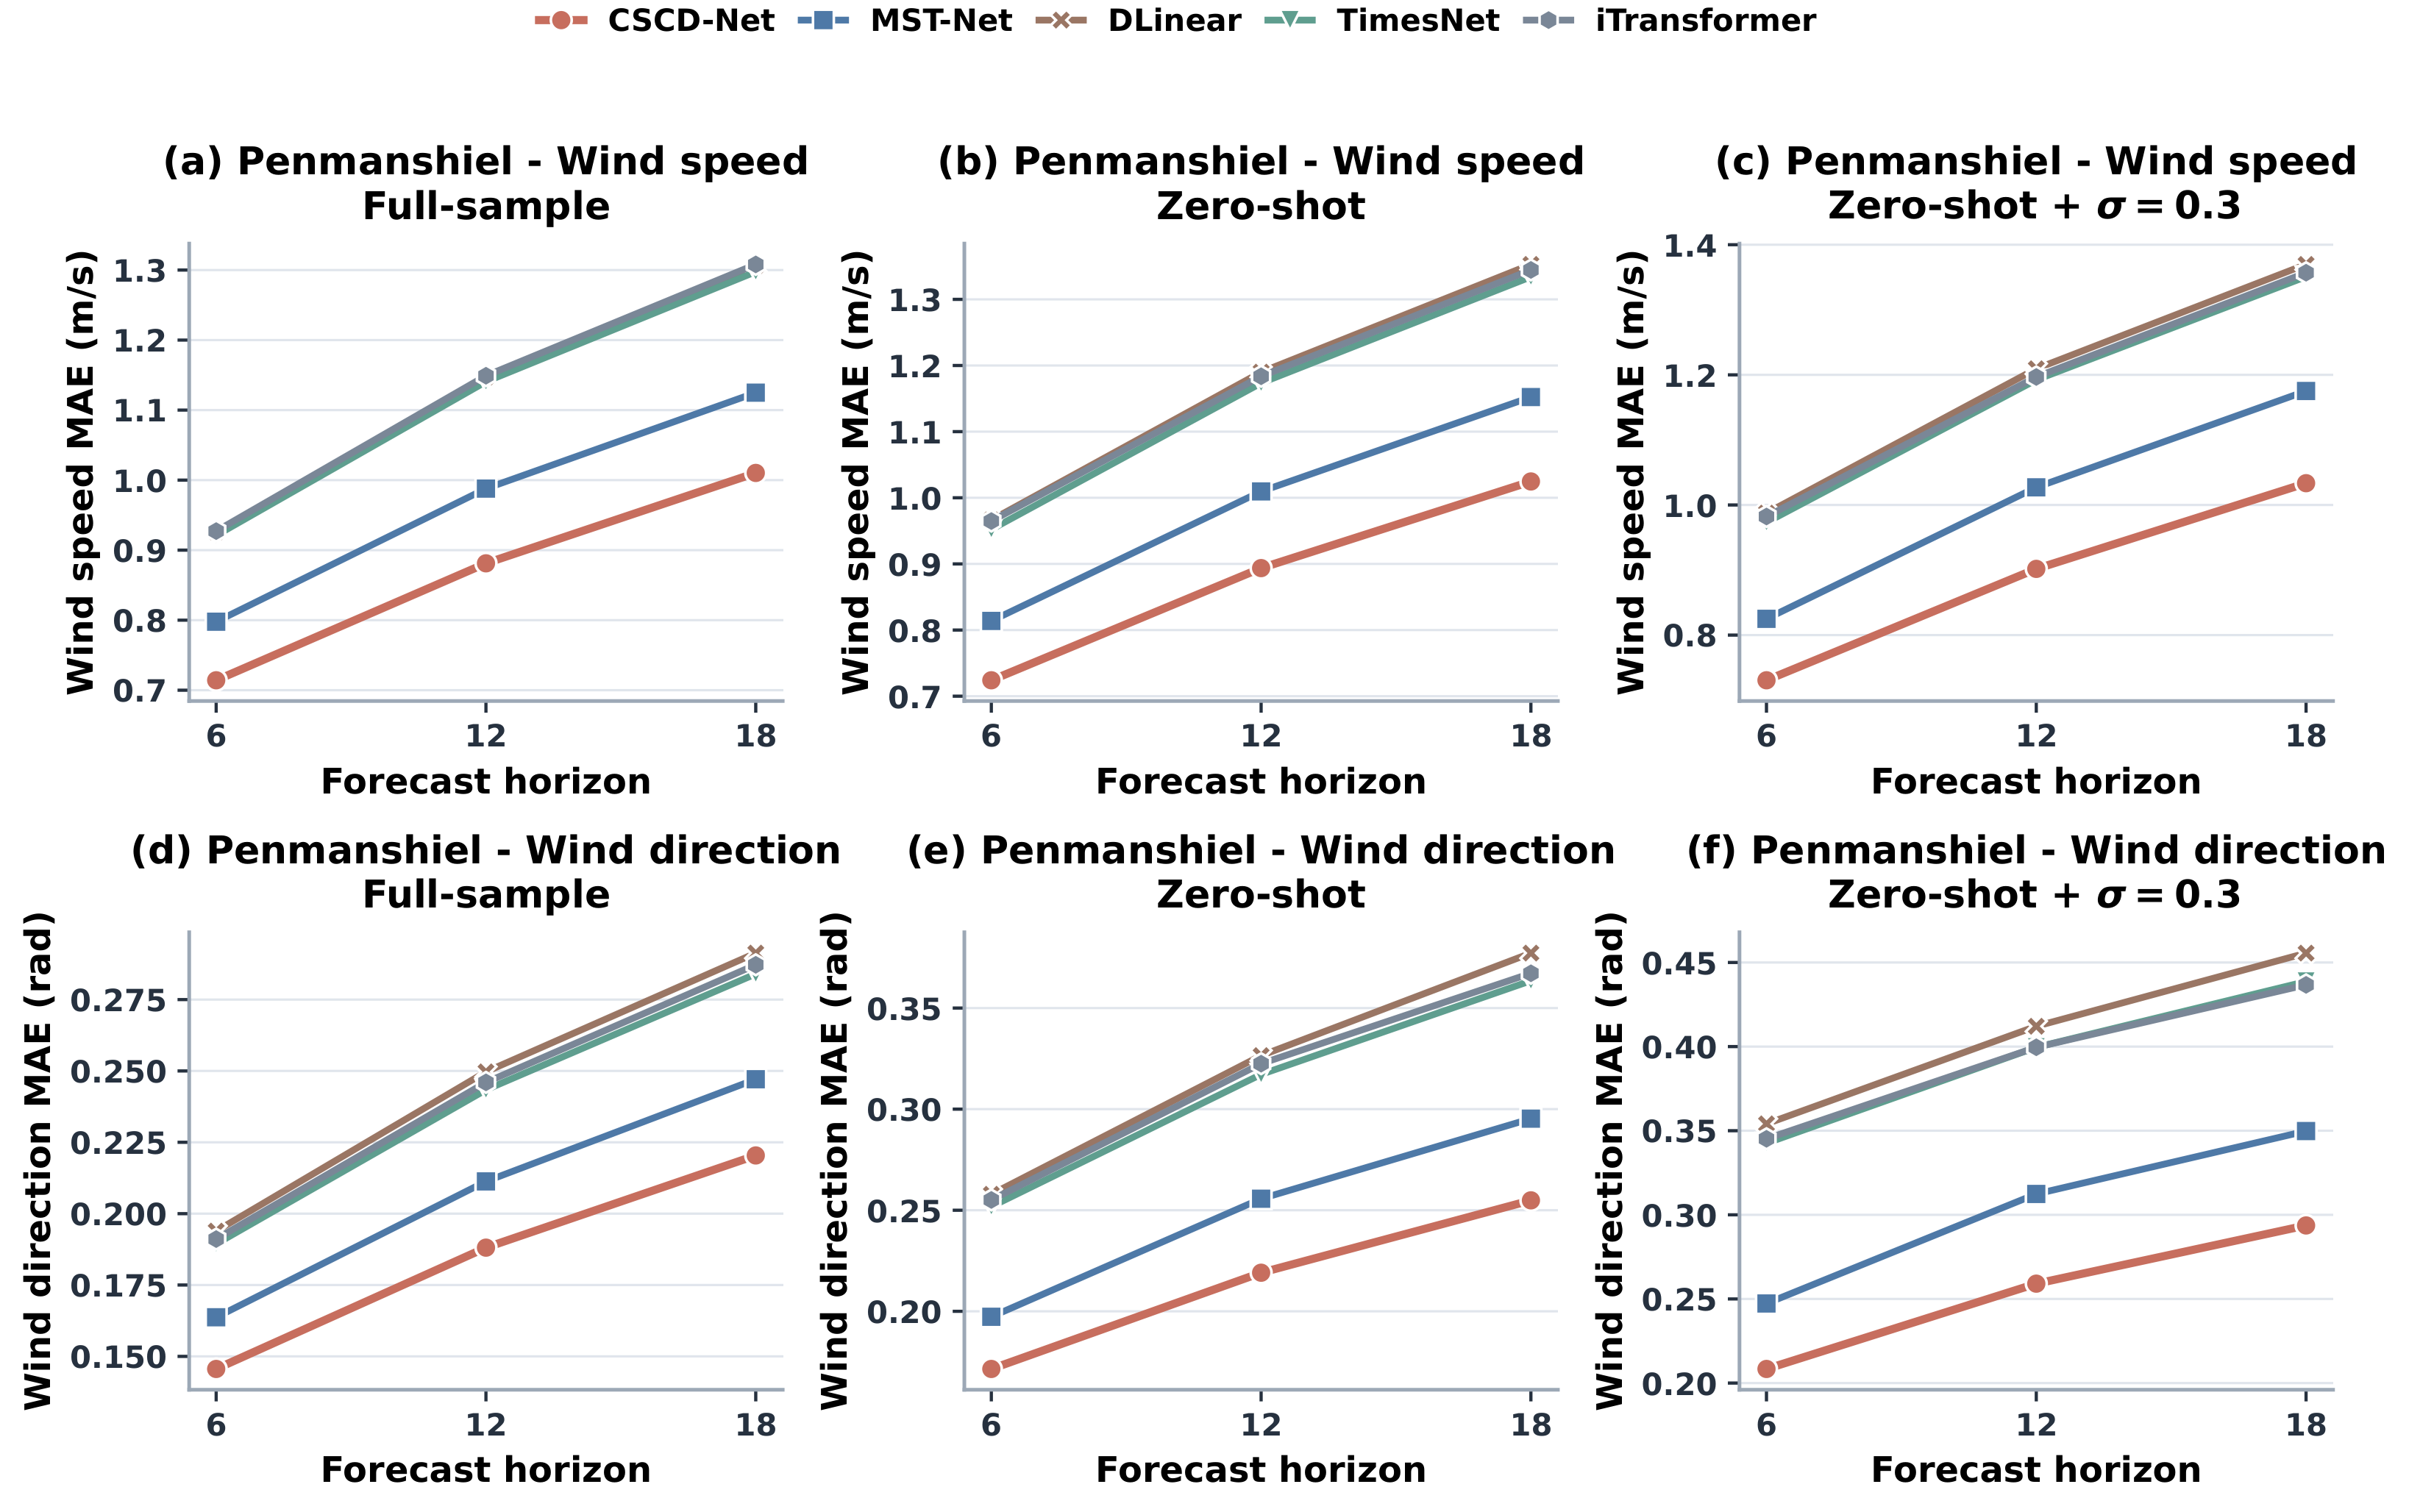
\includegraphics[width=0.48\textwidth]{figures/supp_sparse_zero_shot.png}
\caption{Sparse Deployment Zero-Shot Evaluation on Penmanshiel. The figure compares full-sample training, zero-shot transfer, and zero-shot transfer under sensor noise across multiple forecast horizons.}
\label{fig:sparse_zero_shot}
\end{figure}

Fig.~\ref{fig:sparse_zero_shot} shows that WindFormer has the smallest zero-shot degradation, with a 17.72\% increase in direction MAE under the clean setting and a 15.61\% increase under 0.3-rad noise.

\subsection{Ablation Analysis}
\label{subsec:ablation}

\begin{table*}[!t]
\caption{Ablation study results for different variants on the Shanxi and Penmanshiel datasets.}
\label{tab:ablation}
\centering
\scriptsize
\setlength{\tabcolsep}{3.2pt}
\renewcommand{\arraystretch}{1.08}
\begin{adjustbox}{max width=\textwidth}
\begin{tabular}{l|cccc|cccc|cccc|cccc}
\toprule
\multirow{3}{*}{Variant}
& \multicolumn{4}{c|}{Shanxi-6steps}
& \multicolumn{4}{c|}{Shanxi-12steps}
& \multicolumn{4}{c|}{Penmanshiel-6steps}
& \multicolumn{4}{c}{Penmanshiel-12steps} \\
\cline{2-17}
& \multicolumn{2}{c}{Speed} & \multicolumn{2}{c|}{Wdir}
& \multicolumn{2}{c}{Speed} & \multicolumn{2}{c|}{Wdir}
& \multicolumn{2}{c}{Speed} & \multicolumn{2}{c|}{Wdir}
& \multicolumn{2}{c}{Speed} & \multicolumn{2}{c}{Wdir} \\
\cline{2-17}
& MAE & RMSE & MAE & RMSE
& MAE & RMSE & MAE & RMSE
& MAE & RMSE & MAE & RMSE
& MAE & RMSE & MAE & RMSE \\
\midrule
WindFormer
& \textbf{0.6367} & \textbf{0.9884} & \textbf{0.2717} & \textbf{0.5530}
& \textbf{0.8025} & \textbf{1.2374} & \textbf{0.3441} & \textbf{0.6525}
& \textbf{0.7142} & \textbf{1.1497} & \textbf{0.1456} & \textbf{0.2914}
& \textbf{0.8812} & \textbf{1.4211} & \textbf{0.1881} & \textbf{0.3686} \\
w/o Learnable Weights
& 0.6754 & 1.0421 & 0.2765 & 0.5601
& 0.8465 & 1.3012 & 0.3495 & 0.6612
& 0.7589 & 1.2185 & 0.1502 & 0.2985
& 0.9325 & 1.5052 & 0.1935 & 0.3768 \\
w/o Direction Vector Rep.
& 0.6502 & 1.0065 & 0.6214 & 1.0851
& 0.8188 & 1.2615 & 0.7245 & 1.2562
& 0.7285 & 1.1712 & 0.4985 & 0.8124
& 0.8985 & 1.4485 & 0.5642 & 0.9351 \\
w/o Wind Vector Cons.
& 0.6612 & 1.0215 & 0.2985 & 0.5921
& 0.8315 & 1.2825 & 0.3852 & 0.7124
& 0.7412 & 1.1921 & 0.1685 & 0.3341
& 0.9125 & 1.4721 & 0.2185 & 0.4215 \\
Phase-Attn to Patch
& 0.6845 & 1.0563 & 0.2798 & 0.5644
& 0.8582 & 1.3155 & 0.3541 & 0.6658
& 0.7695 & 1.2312 & 0.1534 & 0.3018
& 0.9458 & 1.5215 & 0.1972 & 0.3812 \\
\bottomrule
\end{tabular}
\end{adjustbox}
\end{table*}

Table~\ref{tab:ablation} validates the contribution of each module. Removing the two-dimensional sine-cosine unit-vector representation mainly harms direction prediction, whereas removing the learnable common-wind weights or replacing Phase-Attention with ordinary patches affects wind-speed prediction more strongly.


\section{Conclusion}
\label{sec:conclusion}

This paper presented WindFormer for joint short-term forecasting of wind speed and wind direction in multi-turbine wind farms. The key idea is to exploit the shared wind-speed field while preserving turbine-specific residual variations, and to transform one-dimensional wind-direction angles into a two-dimensional sine-cosine unit-vector representation that preserves boundary information.

Extensive experiments on two SCADA datasets showed that WindFormer achieved the best overall performance across all forecasting horizons. In the full-sample setting, it consistently outperformed representative baselines on both wind speed and wind direction, with an average error reduction of 8.2\% over the strongest competing model. In the sparse-deployment zero-shot setting, WindFormer also maintained strong cross-turbine generalization: wind-speed degradation remained small, with only about 3.7\%--4.0\% increase on Penmanshiel and near-zero to 1.1\% increase on Shanxi, while wind-direction degradation was also reduced compared with competing methods. These results indicate that explicitly separating common speed dynamics from two-dimensional direction-vector learning is effective for wind farm forecasting.

A current limitation is that the study focuses on short-term SCADA forecasting under two wind-farm scenarios. Future work will extend the model to longer-horizon prediction, more diverse wind farms, and changing turbine availability under more complex meteorological conditions.

\nocite{*}
\bibliographystyle{IEEEtran}
\bibliography{references}

\end{document}
